%\documentclass[man,floatsintext,donotrepeattitle]{apa6}
\documentclass[man,donotrepeattitle]{apa6}

% http://tex.stackexchange.com/questions/279/how-do-i-ensure-that-figures-appear-in-the-section-theyre-associated-with
\usepackage{placeins}

\usepackage[nodayofweek]{datetime}% http://ctan.org/pkg/datetime
\usepackage{xfrac}
\usepackage{textcomp}
\usepackage[american]{babel}
\usepackage[utf8]{inputenc}

% Single space after period (Mike prefers)
\frenchspacing

% http://tex.stackexchange.com/questions/36423/random-unwanted-space-between-paragraphs
\raggedbottom

% Changing horizontal space between subsubsection title and text, without loading titlesec package.
% Not loading titlesec because it clashes with apa6 package.
% Took base \@startsection command from apa6 .cls file, and tweaked horizontal spacing. 
% http://tex.stackexchange.com/questions/22576/redefining-sectioning-commands
% http://www.tex.ac.uk/cgi-bin/texfaq2html?label=atsigns
% http://tex.stackexchange.com/questions/60127/subsubsection-description-and-title-not-separated
\makeatletter
\renewcommand{\subsubsection}{%
  \@startsection
  {subsubsection}%
  {3}%
  {\parindent}%
  {0\baselineskip \@plus 0.2ex \@minus 0.2ex}%
  {-.4em}%
  {\normalfont\normalsize\bfseries\addperi}}
\renewcommand{\paragraph}{%
  \@startsection
  {paragraph}%
  {4}%
  {\parindent}%
  {0\baselineskip \@plus 0.2ex \@minus 0.2ex}%
  {-.4em}%
  {\normalfont\normalsize\bfseries\itshape\addperi}}
\makeatother

% ref: http://tex.stackexchange.com/questions/28516/how-to-change-the-title-of-toc
\addto\captionsamerican{% Replace ``english'' with the language you use
  \renewcommand{\contentsname}%
  {Table of Contents}%
}

%\usepackage[compact]{titlesec}
\usepackage{tabu}
\usepackage{amssymb,amsmath}
\usepackage{setspace}

% ref: http://tex.stackexchange.com/questions/48509/insert-list-of-figures-in-the-table-of-contents
\usepackage[nottoc,numbib]{tocbibind}

\usepackage[hyphens]{url}

% ref: http://tex.stackexchange.com/questions/73862/how-can-i-make-a-clickable-table-of-contents
\usepackage{hyperref}
\hypersetup{
  colorlinks,
  citecolor=black,
  filecolor=black,
  linkcolor=black,
  urlcolor=black
}
%\hypersetup{linktocpage}

%\usepackage{breakurl}
\usepackage{subfigure}
\usepackage{graphicx}

\usepackage[group-separator={,}]{siunitx}
\newcommand{\numNoZero}[1]{{\sisetup{add-integer-zero=false}\num{#1}}}

\RequirePackage[l2tabu, orthodox]{nag}
\graphicspath{{./figures/dissertation/}} % Specifies the directory where pictures are stored

\usepackage{csquotes}
\usepackage[style=apa,sortcites=true,sorting=nyt,backend=biber,doi=false,uniquename=false]{biblatex}
\DeclareLanguageMapping{american}{american-apa}

\addbibresource{bibliography.bib}

% Needed to ensure periods are placed at the end of every bibliography entry in the references section
\AtEveryBibitem{\clearfield{doi}}

% http://tex.stackexchange.com/questions/55780/disable-month-in-biblatex-bibliography
\AtEveryBibitem{\clearfield{month}}
\AtEveryCitekey{\clearfield{month}}

% Make sure only urls that are printed in references section are for webpages
\AtEveryBibitem{
  \ifentrytype{misc}{}{
    \clearfield{url}
  }
}

% ref: http://tex.stackexchange.com/questions/128592/remove-backslashes-from-url-fields-in-bib-entry
\DeclareSourcemap{
  \maps[datatype=bibtex]{
    \map{
      \step[fieldsource=url,
	match=\regexp{\\},
      replace=\regexp{}]
    }
  }
}

% Do not let biblatex change any of the casing in the bibliography file
\DeclareRobustCommand{\MakeSentenceCase*}[1]{{#1}}

% If the toc is too detailed, try limiting the depth of printed sections in the TOC:
\setcounter{tocdepth}{2}

\title{Comparing vector-based and ACT-R memory models using large-scale datasets:\protect\\User-customized hashtag and tag prediction on Twitter and StackOverflow}
\shorttitle{Comparing memory models of tag retrieval}
%\shorttitle{}

\author{Clayton Stanley and Michael D. Byrne}
\affiliation{Rice University}

\leftheader{Beitzel}

\keywords{ACT-R declarative memory theory, vector-based models, LSA, machine learning}

\begin{document}

\abstract{
  The growth of social media and user-created content on online sites provides unique opportunities to study models of declarative memory.
  The tasks of choosing a hashtag for a tweet and tagging a post on StackOverflow were framed as declarative memory retrieval problems.
  Two state-of-the-art cognitively-plausible declarative memory models were evaluated on how accurately they predict a user's chosen tags: an ACT-R based Bayesian model and a random permutation vector-based model.
  Millions of posts and tweets were collected, and both declarative memory models were used to predict Twitter hashtags and StackOverflow tags.
  The results show that past user behavior of tag use is a strong predictor of future behavior.
  Furthermore, past behavior was successfully incorporated into the random permutation model that previously used only context.
  Also, ACT-R's attentional weight term was linked to a common entropy-weighting natural language processing method used to attenuate low-predictor words.
  Word order was not found to be strong predictor of tag use, and the random permutation model performed comparably to the Bayesian model without including word order.
  This shows that the strength of the random permutation model is not in the ability to represent word order, but rather in the way in which context information is successfully compressed.
  Finally, model accuracy was moderate to high for the tasks, which supports the theory that choosing tags on StackOverflow and Twitter is primarily a declarative memory retrieval process. 
  The results of the large-scale exploration show how the architecture of the two memory models can be modified to significantly improve accuracy,
  and may suggest task-independent general modifications that can help improve model fit to human data in a much wider range of domains.
}

%\note{\today}

\maketitle

%\newpage

\section{Chapter 1: Introduction}

The ACT-R cognitive architecture \parencite{Anderson2007} contains one of the leading theories of human cognitive processing.
The declarative memory component in ACT-R is a Bayesian statistical model.
This is the same type of co-occurrence-based Naive Bayes statistical model that is prominent in the more general machine learning field.
When these Bayesian models are used for machine learning, it is common to use a large number of observations to construct the co-occurrence matrix that is the foundation for the model.
The primary reason for this is that the stability of statistical models increase as sample size increases.

However, it is much less common in the cognitive modeling community to use a large number of observations to build up declarative memory when creating ACT-R models.
If a cognitive modeler is using the declarative memory component of ACT-R,
it is common to either construct the co-occurrences by hand, or use a small training set of data to initially build up the declarative memory system.
This approach can and has worked well.
Essentially, the modeler is only including the observations in declarative memory that are relevant to the specific task that they are studying.

However, this approach is problematic for two main reasons:
First, it means that the declarative memory system for every developed model must be hand crafted and customized for that model, which takes enormous time and effort.
Second, it means that modelers are continuing to use small sample sizes for the declarative memory components in their models.

This has important implications for understanding declarative memory:
First, it is difficult to verify and explore modifications to the declarative memory architecture because the datasets are not large enough or rich enough to rigorously test modifications to the theory.
It also means that we do yet fully understand how well the ACT-R declarative memory theory scales when the number of chunks begins to approach the number of chunks that are actually stored in human declarative memory.

There is, however, an opportunity to change this approach.
With the massive growth of human-created content on social media sites (e.g., Twitter, StackOverflow, Wikipedia), and public access to many of those databases,
it is now possible to evaluate psychological theories of declarative memory on large-scale real-world tasks where the theory can be tested on hundreds of millions to billions of data points.
This will provide a way to test if these models scale, and evaluate the psychological validity of these models as the number of observations used increases by orders of magnitude.

A few researchers have started to use these large databases to evaluate how well declarative memory models scale,
for both ACT-R Bayesian models \parencites{Fu2007,Pirolli2003,Stanley2013,Douglass2010} and vector-based memory models \parencites{Jones2007,Rutledge2008,Recchia2010,Sahlgren2008}.

The work in this study expands on previous work that has tested retrieval models on large-scale datasets.
It focuses specifically on how two state-of-the-art declarative memory retrieval models (ACT-R Bayesian and vector-based) can be improved by testing these models on two real-world tagging tasks.
One primary objective is to compare the random permutation vector-based model to ACT-R's declarative memory theory when large datasets are used for each model. 
Another objective is to improve each model, and measure how incorporating the strengths of each model into the other (i.e., modifying model components) influences accuracy.
For example, it is currently unexplored how a vector-based model can be modified to retrieve results that are based not only on context, but also on the prior odds that a particular item in memory will be needed again.
Large-scale datasets were used throughout the model development and evaluation process.
This provides an ideal testing environment for constraints and assumptions for each theory to be rapidly tested and new model components to be hypothesized and quickly evaluated.

\subsection{Research Questions}

The core question motivating this research is:
What kinds of cognitively-plausible models can best predict the tags that a user on a social media site uses?
This question can be tested by generating a prediction for the most likely used hashtag whenever a user is about to generate a hashtag, and then comparing the user's chosen hashtag to the model's prediction.
This process can be framed as a memory retrieval problem.
The process of suggesting a relevant hashtag to a user can be thought of as a memory retrieval request for a hashtag, given prior hashtag use and current context.

Co-occurrence-based modeling has been shown as a potentially useful approach when predicting Twitter hashtag use \parencite{Efron2010} and StackOverflow tag use \parencites{Stanley2013}.
Several memory retrieval models are based on this broad methodology, where a count is maintained of the times each contextual element (such as a word in a post) co-occur with a tag.
At least two of the current memory retrieval models are based on a co-occurrence methodology:
ACT-R's declarative memory (DM) retrieval theory and random permutation vector-based memory systems.

\subsubsection{StackOverflow and Twitter}

These two memory systems were compared across two domains where users generate tags for posts: Twitter and StackOverflow.
Twitter is a microblogging service where users create 140 character ``tweets'' and broadcast those messages out to the users who follow their posts.
A user is free to annotate important concepts or words in the tweet by preceding words with ``\#,'' thereby making the word into a hashtag.
After the tweet is created the hashtags become hyperlinks, and if clicked on will take a user to a summary feed of all of the tweets across Twitter that have used that hashtag.
Some recent and often used hashtags for Twitter are \emph{\#photography}, \emph{\#startup}, \emph{\#4change}, \emph{\#android}, and \emph{\#solar}.

The two memory retrieval models were also tested on tag use for StackOverflow posts.
StackOverflow is a question and answer site for computer programming where users ask programming-related questions and fellow members of the community provide answers.
A user with a programming-related question creates a post with their question and tags the post with a few specific programming-related tags. 
The tags chosen by a user on the StackOverflow site represent the primary topic of the question, such as a specific programming language, tool, software package, or framework.
Some example tags for StackOverflow are \emph{PHP}, \emph{Arrays}, \emph{MVC}, \emph{C\#}, and \emph{Common Lisp}.

The StackOverflow and Twitter datasets were chosen because the human-created content between them is quite different, and I am interested in retrieval models that generalize across tasks.
However, they are also similar on several accounts:
Both domains have amassed large amounts of user-created content, users generate tags for posts when creating content on the site (hashtags for Twitter and tags for StackOverflow),
and the user data from the datasets are publicly available for analysis.

\subsection{Roadmap}

This document is separated into 7 chapters.
Chapter 1 introduced the declarative memory research and motivated why it is interesting both from a theoretical and applied perspective to evaluate declarative memory models on large-scale datasets.
The task to test the models was also introduced: tagging of user-generated content on StackOverflow and Twitter.
Chapter 2 describes the vector-based and Bayesian declarative memory models that will be evaluated in this research, and shows how these models are related to the other common declarative memory models that are studied.
Chapter 3 presents the overall method for testing the models on the StackOverflow and Twitter datasets.
Chapter 4 shows the results for the first test of the models, where the model term for past user behavior is examined in isolation, and tags are predicted based purely on a user's past tagging history.
Chapter 5 adds the context component to the models, and shows how model accuracy is influenced by changing various architectural components of each model.
Chapter 6 describes model results when prior and context are combined and tested on both of the dataset subsets used for Chapter 4 and Chapter 5.
Finally, Chapter 7 provides a general discussion of the overall findings.

\section{Chapter 2: Theoretical Background}

The ACT-R declarative memory theory and the vector-based retrieval models will be described.
The Latent Semantic Analysis (LSA) theory is closely related to vector-based retrieval models, so an overview of LSA will also be included.
The theories underlying the ACT-R and vector-based models will be compared.
Also, different tagging models have already been applied to various recommendation systems to tag user-generated content.
Many of these models are based on the same Bayesian statistical framework that is the foundation of the ACT-R declarative memory theory.
So these systems will be described and the models used will be discussed within the context of Bayesian statistical models, LSA approaches, and the ACT-R declarative memory theory. 

\subsection{ACT-R Declarative Memory Theory}

ACT-R \parencite{Anderson2007} is a cognitive architecture that formalizes how each cognitive process of the mind (e.g., memory, learning, visual and motor) interacts to produce behavior.
The declarative memory system is a component of that architecture that models the timing, learning, and forgetting processes that make up declarative memory storage and retrieval.
The equations that make up this system were derived from a rational analysis of declarative memory retrieval.
That is, given the task of retrieving a chunk of information from declarative memory,
the current context (i.e., external and internal environment state), and past experience (i.e., prior memories and exposure), 
what is the optimal behavior (i.e., the optimal chunk to retrieve from memory)?
Using Bayesian reasoning, each chunk of information in declarative memory can be assigned a prior likelihood of needing retrieval again, given the prior history of exposure to the chunk.
These chunk prior probabilities are then adjusted for the current context, so that the posterior probabilities represent the likelihood that a chunk is needed, given prior odds and adjusted by current environment state.

\subsection{Latent Semantic Analysis Memory Theory}

Latent Semantic Analysis \parencite{Landauer1997} (LSA) is an alternative representation of declarative memory.
Both ACT-R's Bayesian declarative memory model and LSA compute activations based on a co-occurrence matrix.
However, LSA performs further processing on that matrix in order to collapse words that have similar meaning.
LSA uses the Singular Value Decomposition process to reduce the dimensionality of the word by document co-occurrence matrix, while maintaining as much of the variance in the original full matrix as possible.
The strength of association between two words is measured by the cosine of the two word vectors across the reduced dimension space.

\subsection{Vector-Based Memory Systems}

``Holographic'' memory systems \parencite{Plate1995} or vector-based memory systems represent a concept (i.e., a chunk) as a vector.
The representation of the concept is distributed across all elements of the vector.
This is somewhat similar to taking a column (i.e., a tag) on a word co-occurrence matrix and viewing the distribution of co-occurrence counts across the rows in the column as the representation of that concept.
However, vector-based memory systems represent information in a much more compact way than a full word co-occurrence matrix.

For vector-based systems, each word is represented by an environment vector $e_{i}$ that is nearly orthogonal to all other words' environment vectors.
The number of dimensions for these vectors is much less than the number of rows in a full word co-occurrence matrix, which is how vector-based systems represent information in a much more compact space.
Paired with each environment vector ($e_{i}$) is a memory vector ($m_{i}$) that contains the summed representation of all other environment vectors that have co-occurred with that $e_{i}$ environment vector.
These memory vectors can contain environment vectors from position-independent word co-occurrence information ($c_{i}$) and word order information ($o_{i}$), which can be combined into a single representation ($m_{i}$).
Over time, memory vectors accumulate a distributed representation of the most common environment vectors that co-occurred with them.

\subsubsection{Addressing Word Order}

One of the strengths of vector-based systems is that word order can naturally be represented alongside word co-occurrence in these distributed representations.
With vector-based systems, order information is included by creating an environment vector ($e_{bind(i,\Phi)}$) that is a function of environment vectors for both the word ($e_{i}$) and location ($\Phi$).
This function has the useful property that the resulting environment vector and the location vector can be inverted to return the original word's environment vector.
Circular convolution and inverse circular convolution (i.e., circular correlation) are used by \textcite{Plate1995} and \textcite{Jones2007}'s BEAGLE model to implement these operations.
This allows for retrieval requests such as ``playing \#$\Phi$,'' ``just read \#$\Phi$,'' and ``vector-based $\Phi$ systems.''

\subsubsection{Random Permutation Model}

In order to represent word order information, a function must be used that converts an environment vector for a set of words and positions (e.g., ``stack $\Phi$'') into a new uncorrelated environment vector.
\textcite{Sahlgren2008} used a simple random permutation method for this operation.

A formal description of the random permutation model in \textcite{Sahlgren2008} is included in Table \ref{tabRandPermModel}.
With random permutations, each word environment vector ($e_{i}$) is a large sparse vector of zeros with a few one and negative one values in random locations. 
In order to create a new environment vector for a word that preceded another word in a sentence, that word's environment vector is shifted to the left one position.
This produces a new environment vector ($e_{i^{-1}}$) for the combination of the word and the position that is uncorrelated with the original word's environment vector and all other environment vectors.

\begin{table}[!ht]
  \caption{Random permutation model}
  \label{tabRandPermModel}
  {\tabulinesep=1.2mm
    \begin{tabu}{ll}
      \hline
      Common Name &  Equation \\
      \hline
      Activation &		$A_{i} = r(m_{C},m_{i})$ \\
      Memory Vector &		$m_{i} = \sum_{i \in all past} c_{i} + \sum_{i \in all past} \sum_{l \in locations} o_{i,l}$ \\
      Unordered Context &	$c_{i} = e_{i}$ \\
      Ordered Context &		$o_{i,l} = e_{i^{-l}}$ \\
      Context Memory Vector &	$m_{C} = \sum_{i \in C} c_{i} + \sum_{i \in C} \sum_{l \in locations} o_{i,l}$ \\
      Environment Vector & 	$e_{i} = rand$ \\
      \hline
    \end{tabu}
  }
\end{table}

\subsubsection{Connection to LSA}

Both vector-based models and LSA calculate word similarity on a reduced matrix.
For LSA, the original word by document matrix is compressed to a factor by document matrix and the number of factors is much less than the number of words.
For vector-based models, each tag is represented by a compressed vector with a length much less than the number of words.

Information is lost with this compression in both cases: by starting with a compressed representation with vector-based models or by reducing to a compressed representation with LSA.
However, the way that the compression works in these two cases is not the same.
LSA uses SVD to find words that have highly correlated tag occurrence distributions (i.e., latent concepts), and then pools those co-occurrence counts into a single dimension.
A vector-based approach like random permutations essentially randomizes the mapping of the words on the reduced set of dimensions, and does not take into account word similarity when generating the mapping.
Nonetheless, vector-based models have been shown to perform similar to if not better than LSA when trained on the TASA and tested on the TOEFL \parencites{Sahlgren2008,Jones2007}.

\subsection{Hashtag Prediction}

Models that attempt to predict a user's chosen hashtag have recently been created and tested for a few social media sites.
Google has even deployed a hashtag recommendation model to help users properly tag posts on their Google+ social media site \parencite{GoogleKeynote2013}.
A tag-suggestion tool has also been deployed for the \url{tex.stackexchange.org} and \url{superuser.com} StackExchange sites.
Models for Twitter and StackOverflow have been proposed and tested, but none have yet been deployed.
Recommendation models for StackOverflow and Twitter will be described in more detail to follow.

\subsubsection{StackOverflow}

\textcite{Stanley2013} used a declarative memory model to predict a user's chosen tags for a post on the StackOverflow site.
They modified the standard ACT-R model in order to more accurately predict tag use on StackOverflow.
A formal description of the modified ACT-R Bayesian model is included in Table \ref{tabModACTRModel}.

\begin{table}[!ht]
  \caption{\citeauthor{Stanley2013}'s StackOverflow tag prediction model}
  \label{tabModACTRModel}
  {\tabulinesep=1.2mm
    \begin{tabu}{ll}
      \hline
      Common Name &  Equation \\
      \hline
      Activation & 		$A_{i} = B_{i} + \sum_{j\in T}^{ } W_{j} S_{ji} + \sum_{j\in B}^{ } W_{j} S_{ji} - O$ \\
      Base Level & 		$B_{i} = log \frac{p_{i}}{1-p_{i}}$ \\
      Strength Assoc. &		$S_{ji} = log \frac{p(i|j)}{p(i))} = log \frac{NN_{ji}}{N_{Row}(j)N_{Col}(i)}$ \\
      Attentional Weight & 	$W_{j} = W \frac{E_{j}} {\sum_{}^{} {E_{j}}} $ \\
      Scaled Entropy & 		$E_{j} = 1-\frac{H_{j}}{H_{max}}$ \\
      Entropy & 		$H_{j} = -\sum_{i=1}^{N}p(i|j)log\left (  p(i|j) \right )$ \\
      \hline
    \end{tabu}
  }
\end{table}

The activation of each tag ($A_{i}$) is a function of four components:
That tag's base-level activation ($B_{i}$), contextual activation for the words in the title, activation for words in the body, and an offset term ($O$).
This model has been modified from the standard ACT-R model in four ways:
Two separate contextual components were used (words in title and body of post), an offset term was added, an entropy measure was used to compute the attentional weight ($W_{j}$),
and the base-level activation of a tag was based on global past tag use and not customized to a user's past tagging history.

The offset term was added to normalize the mean activation across retrievals.
This allowed the use of a logistic regression statistical technique to calibrate the weights for each of the terms.
The scaled entropy measure $E_{j}$ was chosen for the attentional weight ($W_{j}$) term because it has a strong theoretical foundation \parencite{Dumais1991} and is parameter free.
Looking at $W_{j}$, if $E_{j}$ is low then $W_{j}$ is low, meaning that the scaled entropy measure helps allocate limited attentional resources to predictive contextual elements.

\subsubsection{Twitter}

Several hashtag recommendation models for Twitter have been developed recently.
One of the first models used a Bayesian co-occurrence statistical technique to predict the most likely hashtag associated with a post as a function of prior hashtag use and context \parencite{Mazzia2009}.
The model presented by \textcite{Mazzia2009} is quite similar to an ACT-R declarative retrieval model.
The main potential difference is that --- like \textcite{Stanley2013} --- the global prior likelihood of a hashtag is computed without taking into account the specific user's past history.

Several other models have taken a tweet-centered approach to hashtag prediction, where suggested hashtags are collected from hashtags used from similar tweets.
\textcites{Li2011, Zangerle2011, Kywe2012} all store a content vector for each tweet, and then compute a word co-occurrence-based similarity score between a composed tweet and the rest of the tweets in the database.

There has been a mix of co-occurrence models created to predict hashtag use on Twitter, and the results are encouraging.
However, there has been little research on how a specific user's past hashtag use should influence the model's prediction when that user is composing a tweet.
\textcite{Kywe2012} did take a user-centered view with their model, but the hashtags predicted by the user and content were analyzed separately and then the top from each group were combined for prediction.
The ACT-R declarative memory retrieval theory shows how past user behavior and current context combine to produce the most likely retrieval.
Each component is summed together to generate a total activation, and then the likelihood of chunks are ranked by that summed activation.
This technique is compensatory and allows for a more natural combination of the two components, where weights can be assigned to each component depending on how strongly each term predicts performance.

\section{Chapter 3: General Methodology}

Each specific result of the research (to be presented in Chapters 4-6) requires a sightly different method to study.
However, there is a common general methodology that applies across all results that will be described first.
Different subsets of the StackOverflow and Twitter datasets were used evaluate past user behavior in isolation and to test the context component of each memory model.
These datasets will be named and described in general terms.
Also, the general methods used to tokenize and stem the words in all of the datasets will be described.

\subsection{Models}

Two models were evaluated for hashtag prediction on both the Twitter and StackOverflow datasets: a vector-based model and Bayesian retrieval model.
The random permutation model \parencite{Sahlgren2008} in Table \ref{tabRandPermModel} was used for the vector-based model,
since it has shown to perform better than the original BEAGLE vector-based model \parencite{Recchia2010}.
The modified ACT-R Bayesian model \parencite{Stanley2013} in Table \ref{tabModACTRModel} was used for the Bayesian model, since it has already been applied to tag use on StackOverflow posts.

The two memory models were evaluated on predicting user-chosen tags for Twitter tweets and StackOverflow posts.
The co-occurrence matrices used for the context component of each model were generated from a large subset of the Twitter and StackOverflow datasets.
Each model was tested by evaluating the accuracy of model-chosen tags on a fresh test subset of the datasets.
Accuracy was assessed by comparing model performance with the human data.

\subsection{Datasets}

The most recent quarterly published StackOverflow dataset \parencite{DataDump2014} was used to test the models on user chosen tags for posts.
This dataset contains around \num{5.7} million posts and \num{34377} unique tags.

Unlike StackOverflow, the entire Twitter dataset is not released to the public.
Due to this and the scale of Twitter, only a part of the Twitter dataset relevant to this research was collected.

\subsubsection{Popular Users Dataset}

A popular-users dataset was collected for both StackOverflow and Twitter.
This dataset consists of all of the tweets and posts from various samples of the top users for each site.
This dataset was collected by fetching all past tagging history for each of the top users.
It was used to explore the growth and decay characteristics of a hashtag for individual users.
The temporal dynamics of ACT-R's decay rate model for a chunk were evaluated against these data.
Multiple samples were taken across a broad range of user types for each dataset to ensure that the model results were not dependent on specific attributes in a single sample.

For StackOverflow, top users were identified by their reputation score on the site (based on their upvoted questions and answers) and the total number of questions asked on the site.
To create the StackOverflow popular-users dataset, a total of 12 slices of users were taken at different levels of reputation and total number of questions asked.
500 users were sampled that had a reputation higher than \num{500}, \num{1000}, \num{5000}, \num{10000}, \num{50000}, and \num{100000}.
100 users were sampled that had asked a total number of questions higher than \num{50}, \num{100}, \num{200}, \num{300}, \num{400}, \num{500}.

For Twitter, top users were those that had the largest number of followers and had authored the largest number of tweets.
To create the Twitter popular-users dataset, 12 slices were also taken, this time at different levels of number of followers and total number of tweets.
100 users were sampled that had a total number of followers higher than \num{1000}, \num{5000}, \num{10000}, \num{100000}, \num{1000000}, and \num{10000000},
and a total number of tweets higher than \num{100}, \num{500}, \num{1000}, \num{5000}, \num{10000}, and \num{50000}.

\subsubsection{Popular Hashtags Dataset}

An additional popular-hashtags dataset was collected for Twitter.
The purpose of this dataset is to test the accuracy of each model's predicted most likely hashtag(s) for a tweet.
The dataset contains approximately three million tweets where at least one of the 400 most popular hashtags are used.
A quota of three million tweets was selected because previously research testing Bayesian co-occurrence models on large-scale datasets has used on the order of one million documents
\parencites{Stanley2013,Douglass2010,Budiu2007}.
Tweets were collected in real time until the tweet quota was reached.

Four popular-hashtags datasets were collected at four different time periods, spanning across one month.
Multiple datasets were collected to ensure that the results were not dependent on a particular sample of hashtags and would generalize across different popular-hashtag datasets and different time periods.
Each dataset required around four days to collect enough tweets to reach the quota, and one collection was done each week.

\subsubsection{Randomly Sampled Dataset}

Since the entire dataset is available for StackOverflow, randomly-sampled posts were used to test the context models rather than creating a popular-tags dataset (analogous to Twitter).
If all Twitter data were available, then the models would have been tested on a randomly-sampled dataset for Twitter as well.
However, since this is not the case for Twitter, the popular-hashtags dataset was used instead of a randomly-sampled dataset for that site,
while models for StackOverflow were tested on the more challenging dataset where posts were randomly sampled across all posts created on the site.

\subsection{Acquiring Datasets}

\subsubsection{StackOverflow}

The entire StackOverflow dataset is packaged and released quarterly to the public.
So the most recent packaged dataset was downloaded and the database tables were imported into PostgreSQL.

\subsubsection{Twitter}

Twitter provides two types of APIs for acquiring data: one based on streaming and a direct query-based interface.
The Tweepy Python package provides a Python functional interface to these APIs, and this package was used to collect data from Twitter.
The query-based interface was used to collect all tweets for specific popular users.
At most \num{3000} of the most recent tweets were collected for each user, since Twitter only allows access to this number of tweets for each user.

The streaming interface was used to collect a sample of all of the tweets that included one of the top 400 hashtags at that time.
Twitter's streaming API only allows at most 400 hashtags to be monitored at a time.
Otherwise a larger number of hashtags would have been collected.
Twitter allows the streaming interface to randomly sample about 1\% of all of the real-time data that is generated on Twitter.
This sampling rate was adequate to collect around three million tweets within a few days.

\subsection{Tokenization}

A custom tokenization algorithm created by \textcite{Owoputi2013} was used to chunk the words in the text.
This algorithm was specifically created for tokenizing Twitter content.
However, during testing it was also found to be robust and well suited for StackOverflow content.
The initial model results with the new tokenizer were qualitatively similar to the model results found in \textcite{Stanley2013} where the Python Natural Language Processing (NLP) toolkit \parencite{Bird2009} was used.
So the same tokenization algorithm from \textcite{Owoputi2013} was used for both StackOverflow and Twitter, since performance was similar to \textcite{Stanley2013} for StackOverflow,
and it seemed beneficial to use the same algorithm for both datasets to make comparisons across datasets more equitable.

\subsection{Stemming}

\textcite{Owoputi2013}'s algorithm handles basic word stemming (e.g., removing ``ed'' and ``ing'' endings), but
with the StackOverflow dataset, it is also possible to convert synonym tags to canonical base tags, since the community maintains a tag-synonym database.
This can be thought of as semantic stemming, where two words with identical meaning are converted to the same canonical word.
So tags used for the post were converted to their root tag when possible.

\section{Chapter 4: Past User Behavior}

How does a user's prior tag use influence their likelihood of choosing that tag in the future?
This question was tested by examining how well ACT-R's base-level activation component of declarative memory predicts the tags that authors choose, given each author's past tagging behavior.
The model predicts that the more recently and frequently used tags have higher prior activations, and are more likely to be needed in the future.

\subsection{Base-level ACT-R model}

The base-level activation component from the full ACT-R declarative memory model is included in Table \ref{tabACTRBLLModel}.

\begin{table}[!ht]
  \caption{Base-level component of ACT-R declarative memory}
  \label{tabACTRBLLModel}
  {\tabulinesep=1.2mm
    \begin{tabu}{ll}
      \hline
      Common Name &  Equation \\
      \hline
      Base-Level Activation &	$B_{i} = log \sum_{j=1}^{n} {t_{j}}^{-d}$ \\
      Optimized Learning &	$B_{i} = log \frac{n}{1-d} - d * log L$ \\
      \hline
    \end{tabu}
  }
\end{table}

Both terms are methods for computing the base-level activation ($B_{i}$) of a chunk in declarative memory.
The standard form has a time dependence and accounts for the fact that the rate of presentations for a given object (e.g., the word ``loop'') can change over time.
The optimized learning form assumes that this rate is constant.

For both equations, $i$ represents each chunk (e.g., the word ``loop''), $j$ is a specific observation for a chunk (e.g., the 2nd time that ``loop'' appears), and $n$ is the number of times each chunk has been observed.
Since the optimized learning form assumes a constant presentation rate for each chunk,
it only has to keep track of the time since the first presentation of a chunk ($L$) and the total number of instances observed for that chunk ($n$). 
It does not have to keep track of the time each specific chunk instance was observed.
Consequently, the optimized learning form of $B_{i}$ is computationally much less expensive than the standard form, and is actually set to the default in the ACT-R Common Lisp implementation.

The decay rate parameter ($d$) represents how fast the activation for an individual presentation of a chunk decays from declarative memory.
Higher values mean that chunk activation decays faster, which means that the most recently presented chunks will have the highest activation, and the total number of times that a chunk has been presented matters less.
Lower decay rate values flip the importance of frequency and recency.

The base-level ($B_{i}$) component in Table \ref{tabACTRBLLModel} is different than the $B_{i}$ used in \textcite{Stanley2013} (Table \ref{tabModACTRModel}).
\citeauthor{Stanley2013} assumed no time dependence, no decay rate, and that the $B_{i}$ is simply a log-odds computation of the probability that each chunk is likely to be presented again, given past frequency.
If a decay rate of 0 is used on the optimized learning form of $B_{i}$, then the equation collapses to $log \left ( n_{i} \right )$,
which is a nonlinear transformation of the $B_{i}$ used by \citeauthor{Stanley2013} ($log \frac{p_{i}}{1-p_{i}}$).
Both forms maintain the same rank ordering, so they should produce similar results.
So the $B_{i}$ component used by \citeauthor{Stanley2013} can be roughly thought of as the standard form of $B_{i}$ when the decay rate is 0 (i.e., a pure frequency model).

\subsection{Method}

The StackOverflow and Twitter popular-users datasets were used to characterize tag growth and decay for a user on each site.
The popular-users dataset contains 12 slices of popular users for both StackOverflow and Twitter.
Each user's tag behavior from the popular-users dataset for each site was analyzed. 

22 different values of the decay rate parameter were explored for each slice
(0, .1, .2, .3, .4, .5, .6, .7, .8, .9, 1.0, 1.1, 1.2, 1.3, 1.4, 1.5, 1.6, 1.8, 2, 5, 10, 20).
The values were chosen to look at how performance changes from a pure frequency model ($d=0$), to a blend of frequency and recency ($d \approx .5$), to a pure recency model ($d=20$).
The decay rate value was varied for both the standard form and optimized learning form of $B_{i}$. 
Only values equal to or below 1 were examined for the optimized learning form, since values above 1 for this form cause a bifurcation and are not psychologically interesting.
The bifurcation occurs because at a decay rate of 1 the denominator of the first term to compute $B_{i}$ goes to zero (see Table \ref{tabACTRBLLModel}).

Both the standard form and optimized learning form of $B_{i}$ were used to predict each user's specific tag history.
To do this, a user's entire tag history was collected, and then each tag instance from oldest to newest was examined.
For each of these tagging instances, the model generated an activation value for each possible tag based on that tag's frequency and recency of past use. 

At each tagging instance, the model has activation values for a set of tags.
Model accuracy was assessed by rank ordering these activations and choosing the model's highest $N$ tags, where $N$ is the number of tags used for that specific post.
The model's chosen $N$ tags were compared to the user's chosen $N$ tags, and if a model's chosen tag was in the set of user's chosen tags, then the prediction was marked as correct.
Otherwise, it was marked as incorrect.

This process was performed across all users in each of the 12 dataset slices for both the Twitter and StackOverflow popular-users datasets.
It was repeated for each of the decay rate values and the two different forms of $B_{i}$.

\subsection{Results}

\subsubsection{Model Performance Across Decay Rate Values}

Looking first at only a single dataset slice, model accuracy for all users in that slice was analyzed.
A plot of the results for one of the 12 slices, for both Twitter and StackOverflow, and for both forms of $B_{i}$ are included in Figures \ref{figPriorSOQSliceDsStd} and \ref{figPriorTwitterSliceDsStd} respectively.

\begin{figure}[!htbp]
  {%
    \setlength{\fboxsep}{0pt}%
    \setlength{\fboxrule}{1pt}%
    \hfill
    \subfigure[][Standard form]{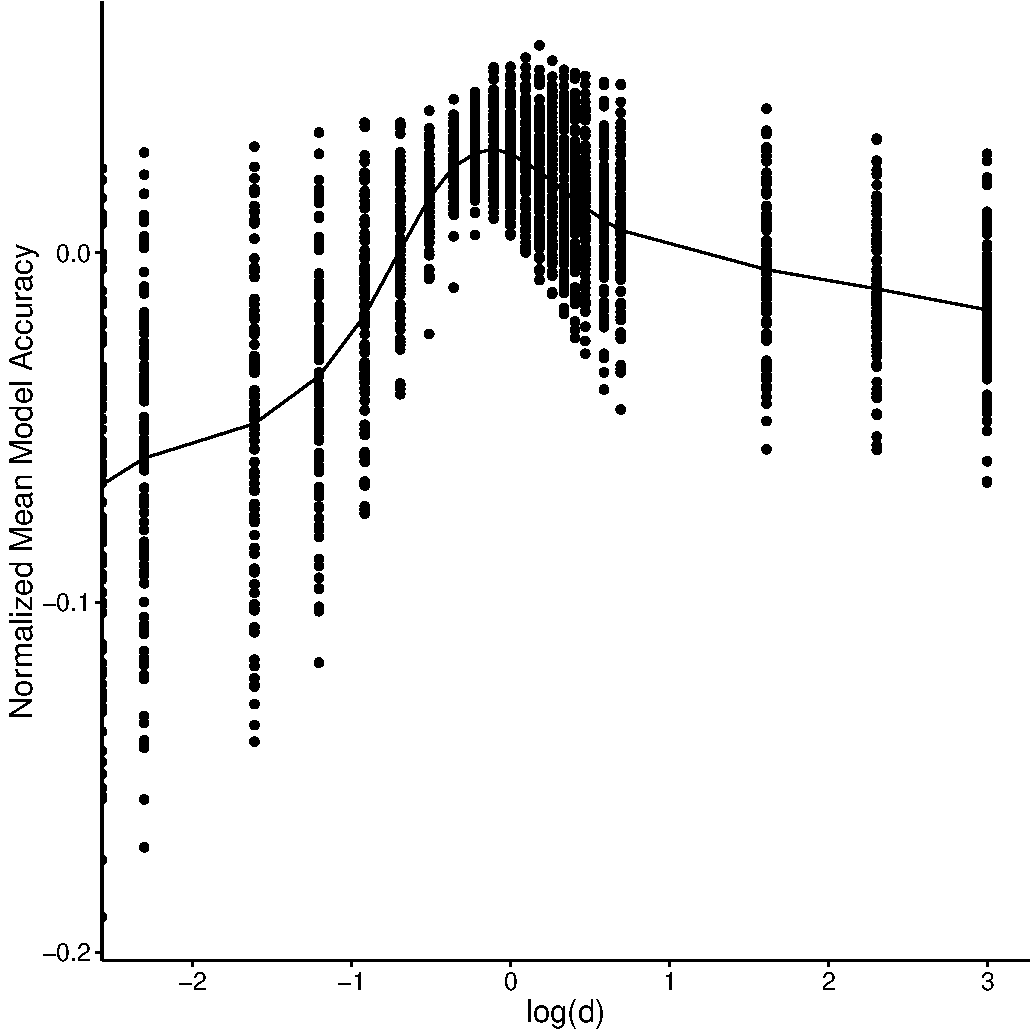
\includegraphics[width=8cm]{visNormMean-SOQgt500r2-topHashtagPostPriorStd-crop.pdf}}
    \hfill
    \subfigure[][Optimized learning form]{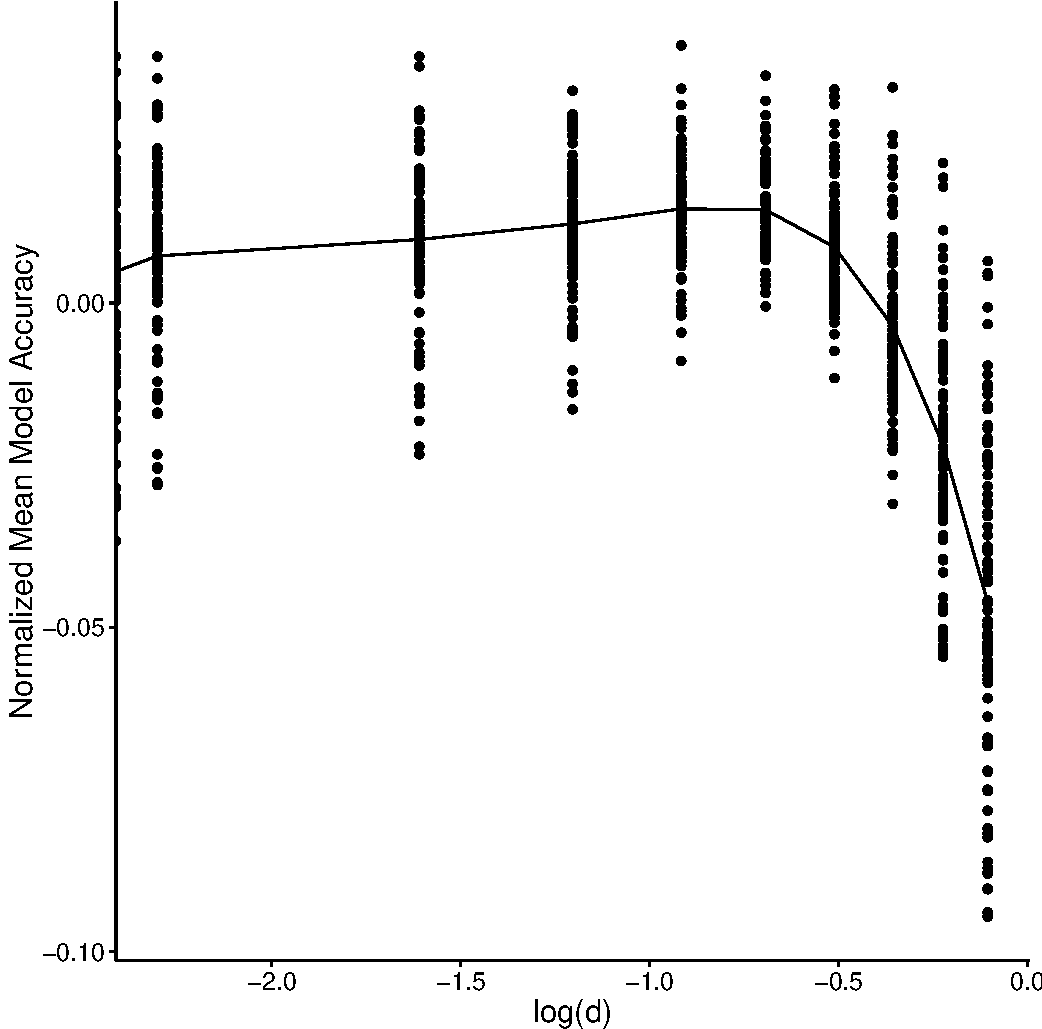
\includegraphics[width=8cm]{visNormMean-SOQgt500r2-topHashtagPostPriorOL2-crop.pdf}}
    \caption{
    Model performance for a single dataset slice for StackOverflow.
    This includes model accuracy as a function of decay rate value for each user in the dataset slice.
    Model accuracy is shown both when the standard from of base-level activation ($B_{i}$) and the optimized learning form of the equation are used. 
  }
    \label{figPriorSOQSliceDsStd}
  }%

\end{figure}

\begin{figure}[!htbp]
  {%
    \setlength{\fboxsep}{0pt}%
    \setlength{\fboxrule}{1pt}%
    \hfill
    \subfigure[][Standard form]{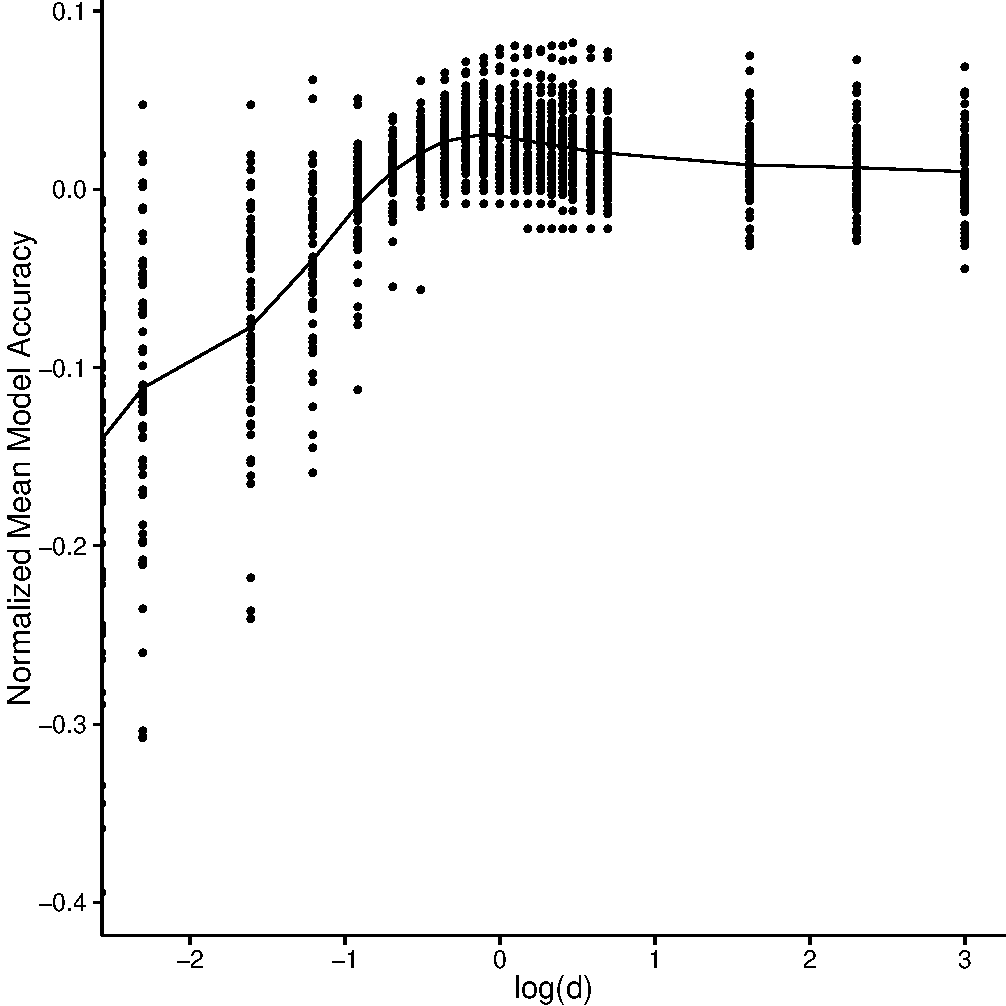
\includegraphics[width=8cm]{visNormMean-TFollowgt10Mr2-topHashtagPostPriorStd-crop.pdf}}
    \hfill
    \subfigure[][Optmized learning form]{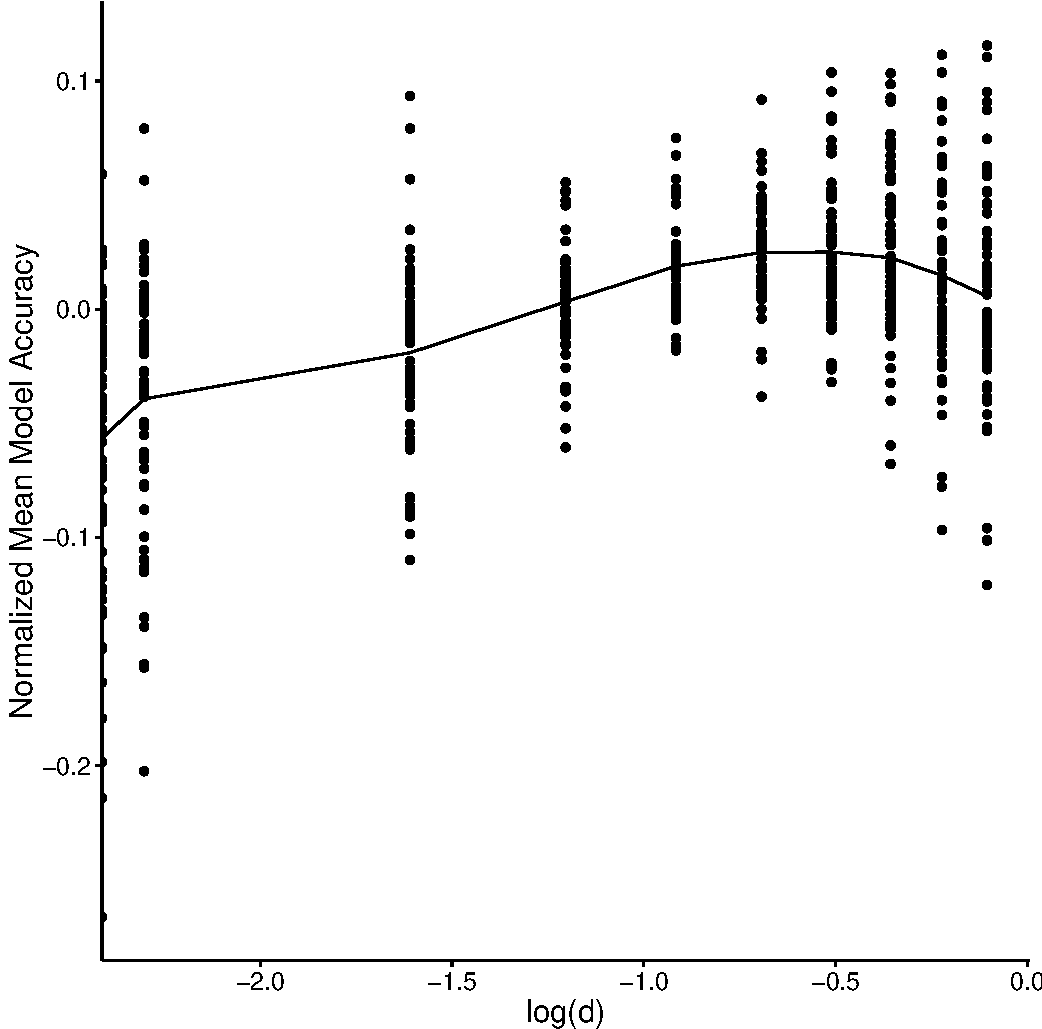
\includegraphics[width=8cm]{visNormMean-TFollowgt10Mr2-topHashtagPostPriorOL2-crop.pdf}}
    \caption{
      Model performance for a single dataset slice for Twitter.
      This includes model accuracy as a function of decay rate value for each user in the dataset slice.
    }
    \label{figPriorTwitterSliceDsStd}
  }%
\end{figure}

Model accuracies at each decay rate value for each user in the dataset slice are included in the plots.
Each user's mean accuracy was subtracted off in order to compute a normalized mean for that user.
This was done so that the relative accuracy change for different decay rate values could be more easily visualized.
The plotting technique is a analogous to what is done when testing the main effect in a repeated measures design (i.e., each subject's mean score is subtracted off).

One large effect in all of the plots is that there is an optimal decay rate value between 0 and 20 that produces the highest model accuracy.
For the standard $B_{i}$ equation, model accuracy for a pure frequency model ($d=0$) is also worse than using a pure recency model ($d=20$), particularly for Twitter.
It makes sense that a pure recency model for Twitter is relatively more accurate than for StackOverflow, as the hashtag lifetime for Twitter is much less than a tag for a programming language on StackOverflow.

When comparing the standard and optimized learning forms of the equation, it is apparent that a pure recency model does not work well for optimized learning.
The best-fit decay rate value for the optimized learning form is also not as clear and pronounced as it is for the standard form (less of a peak).
And the relative accuracy gained from using a pure frequency based model to a blend of frequency and recency is less for the optimized learning form than the standard form of $B_{i}$.

\subsubsection{Aggregate Model Performance}

Aggregate best-fit decay rates were computed by taking the median of all user's best-fit decay rate values across all dataset slices.
The median was used since there were users in the popular-users dataset that did not have enough observations to generate stable predictions, and best-fit decay rate values for these users could be as high as 20.
Using the median effectively trims these unstable values from the sample, without having to define a cut point for an outlier removal process.

Aggregate best-fit decay rate values for each model are included in Figure \ref{figPriorDecay}.
Decay rate values that produced the most accurate model performance are lower for the optimized learning form (\num{.43}) of $B_{i}$ compared to the standard form (\num{.80}).
The optimal values for optimized learning are near \num{0.5}, which lines up with default value used in ACT-R.
So the decay rate values for the standard form are slightly higher than the default values used in ACT-R, but the values found when optimized learning is used line up nicely with the ACT-R defaults.

\begin{figure}[!htbp]
  \scalebox{.8}{\resizebox{\linewidth}{!}{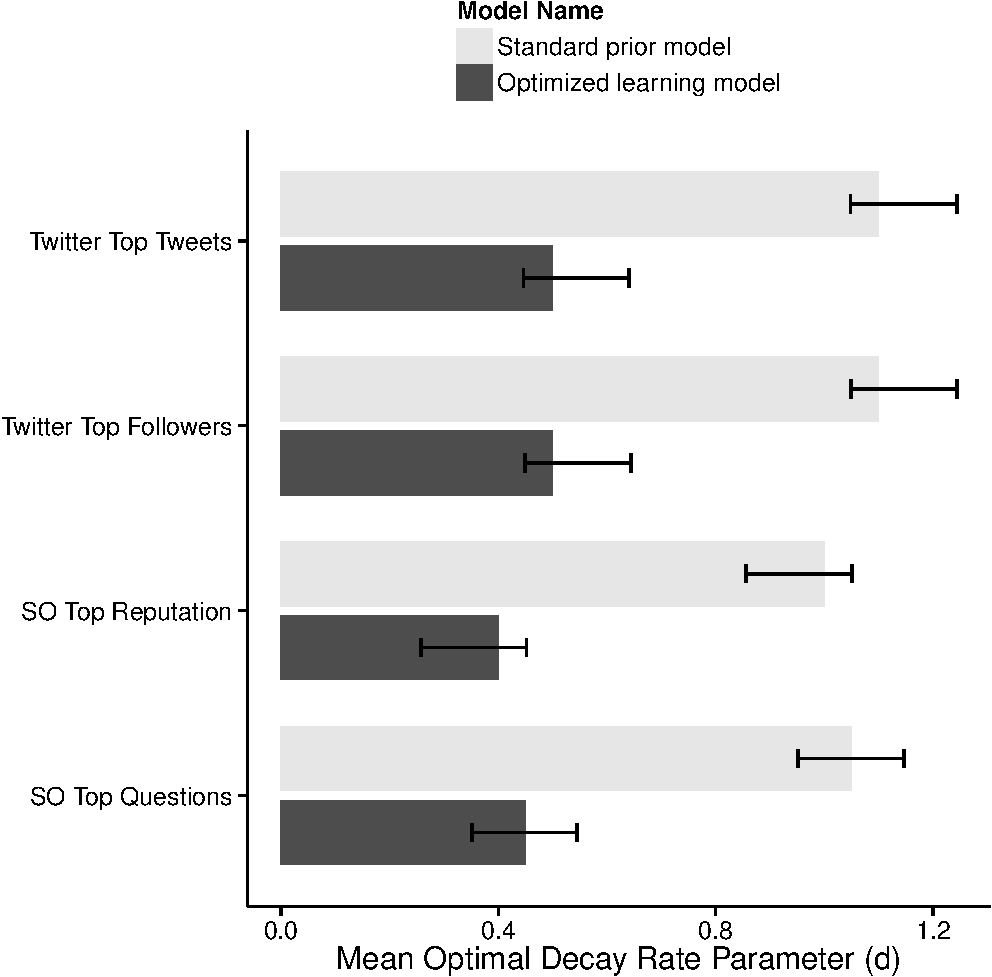
\includegraphics{compareMeanDV-d--crop.pdf}}}
  \caption{
  Overall best-fit decay rate for StackOverflow and Twitter.
  Results are shown for the two Twitter and StackOverflow (SO) popular-users datasets.
  Error bars represent the 95\% bootstrapped confidence interval for the median.
}
  \label{figPriorDecay}
\end{figure}

\FloatBarrier

Finally, model accuracy was analyzed across all dataset slices for StackOverflow and Twitter.
This was done by examining model accuracy at a specific decay rate value for each model.
Accuracy was assessed at each model's previously-determined best-fit values (\num{.43} and \num{.80} for the optimized learning and standard form) and the standard form's default value (\num{0.5}).
Since decay rate values were explored at \num{0.1} increments between the 0 and 1 range, the decay rate values used to examine model accuracy were rounded to the nearest decay rate value that was included in the run.
So a best-fit value of \num{.4} was used for the optimized learning model instead of the \num{.43} average found from the dataset slices.
Accuracy for both sites is included in Figure \ref{figPriorAcc}. 
Aggregate accuracy was computed by taking the mean of every user's model accuracy across all users in all dataset slices.

\begin{figure}[!htbp]
  \scalebox{.8}{\resizebox{\linewidth}{!}{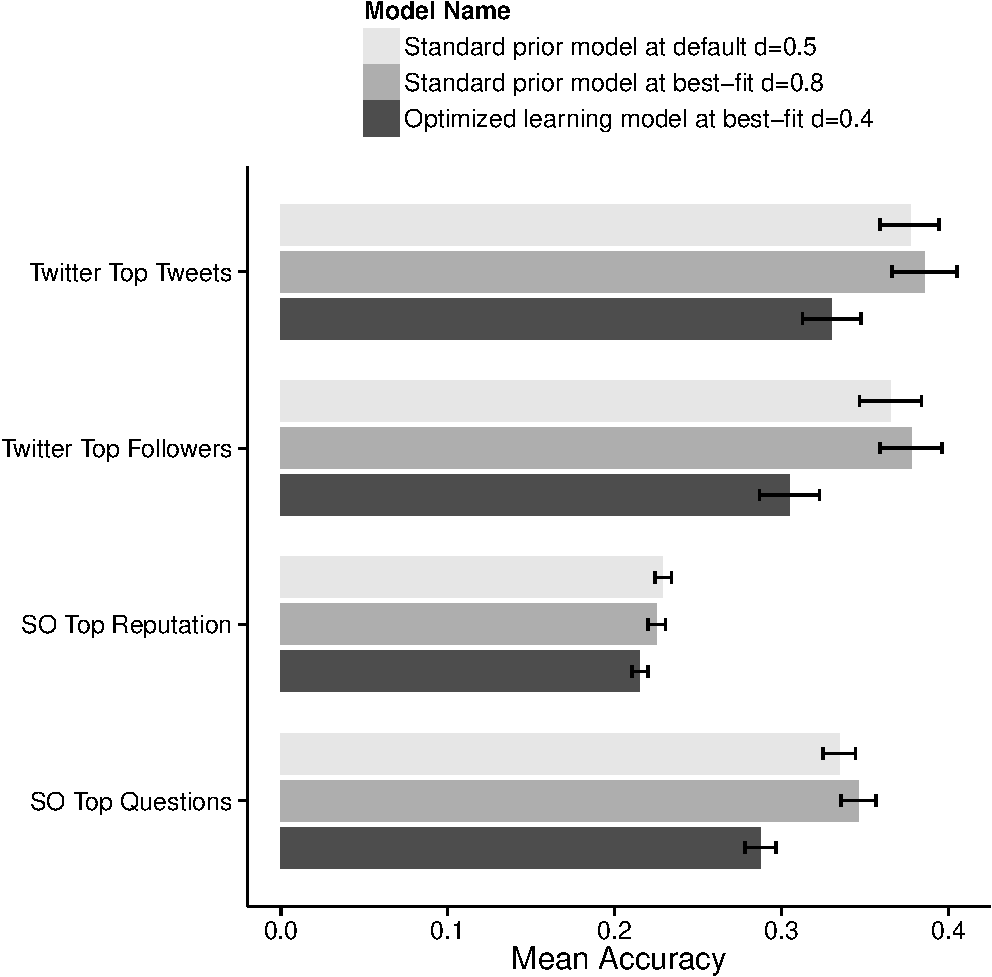
\includegraphics{compareMeanDV-acc--crop.pdf}}}
  \caption{
    Overall model accuracy for StackOverflow and Twitter at optimal decay rate values.
    All error bars are the 95\% bootstrapped confidence interval for the mean. 
  }
  \label{figPriorAcc}
\end{figure}

Accuracy for the standard form (\numNoZero{.33}) is higher than the optimized learning form (\numNoZero{.28}).
This makes sense given that the standard form does not assume equal presentation rate for each chunk, and hashtags on Twitter in particular show trends of high rate of use and then shift to low rate of use. 
The standard form of $B_{i}$ is able to more accurately account for these trends.

ACT-R sets the default decay rate value to \num{0.5}, and the best-fit value for the standard form is higher (\num{0.8}) for these datasets.
The figure shows that although model accuracy does slightly improve for the standard form when increasing the decay rate parameter from \num{0.5} to the optimal value,
that percentage improvement is not as large as the improvement gained from using the standard form compared to the optimized learning form.
Nonetheless, model accuracy is highest when both the standard form is used and the decay rate value is increased. 

\subsection{Discussion}

Given the large tag space used by post authors on StackOverflow and Twitter, it was surprising that model performance is respectable even when only past tag history and no context is used.
This speaks to the importance of taking into account overall past tagging history, and ensuring that the prior component of activation for each tag is customized to each user's specific past tagging history.

Also apparent for these datasets is that the optimized learning form of $B_{i}$ is not as accurate as the standard form.
Further, for the optimized learning form there is not much difference between using a pure frequency-based model and a model where frequency and recency are optimally blended.
This makes sense given that the optimized learning equation in Table \ref{tabACTRBLLModel} collapses to a pure frequency model as the amount of time since the presentation of the first recorded chunk instance increases,
and also since the timespan of recorded tag use for StackOverflow and Twitter is large (years).

So it may be worthwhile to use the standard form instead of the optimized learning form when declarative memory is modeled across a broader range of tasks.
However, this should not be taken as a strong recommendation,
since the performance benefits seen in this study could simply be due to the fact that the declarative memory retrievals span across a large period of time, which is not the case for all tasks.
Nonetheless, the only real reason not to use the standard form is due to computational resource limitations.
Since this is becoming less of an issue as hardware speed increases, it may be time to reconsider the default form of base-level learning used in ACT-R.
It may be the case that the optimized learning form of the equation is no longer computationally necessary.
And if the standard form is used as the default (or simply tried in another experiment),
the results from this study suggest that the optimal decay rate value should be set slightly higher (\num{0.8}) than the default when optimized learning is used (\num{0.5}).

\section{Chapter 5: Combining Predictors}

The declarative memory models analyzed for this research consist of two main components: past behavior and context.
Past tag use was isolated in the first study to see how well ACT-R's prior component of declarative memory (i.e., base-level learning) fits each user's tag use over time.
For the rest of the studies the past behavior and context declarative memory components were combined as well as looked at in isolation.

Chapter 5 will examine how model accuracy is influenced by four architectural concerns
(method of handling stop words, influence of dataset size, method to combine prior and context, and word order).
The four architectural concerns were examined for the following reasons:
During exploratory evaluation, model accuracy seemed to be highly sensitive to the method of dealing with the commonly-used stop words, so several different methods were examined in more detail.
Due to research from \textcite{Budiu2007} and \textcite{Recchia2010}, model accuracy for the Bayesian and vector-based models is influenced by the number of documents in the dataset,
so the effect of dataset size on accuracy was examined in more detail.
One of the primary goals of this research is to identify the best method to combine the model term for past user behavior with the context term for the random-permutation model,
so two different ways to add the model terms were tested.
Finally, previous research has shown that including word order in the vector-based models improves performance \parencites{Jones2007, Sahlgren2008},
so word order was also examined to see if the effect could be replicated and also to measure the overall importance of word order on model accuracy relative to other architectural manipulations.

\subsection{Overall Method}

\subsubsection{Logistic Regression}

In order to best combine these predictors, a logistic regression statistical technique similar to \textcite{Stanley2013} was used to determine the most optimal weights for each term.
When a user creates a tag for a post, a retrieval request for the model is made.
For each request, the model returns a set of tags (all tags that have been observed for that user in the past) and activations associated with each tag.
An activation value is computed for each model component (e.g., prior tag use, context) for each tag.
These values are recorded, and tag instances that match what the author actually tagged are marked as a 1, while all others are marked with a 0.
This process is repeated across all posts where a user chooses a tag, and across all users in the dataset.
Once all of the results are aggregated, a logistic regression is run where the optimal weights for each model component are found that maximize the model's ability to correctly label tags as 0 or 1 based on total activation.

Model accuracy was evaluated by rank ordering all recorded tags by model activation using the optimal weights,
asking the model to tag the top N posts with a 1 (where N is the total number of recorded tagging instances in the dataset sample),
and then comparing the model's chosen tags with the used tags for each post (i.e., looking at the ``hits'').
This is equivalent to throttling the threshold in the logistic regression such that the total number of observations labeled as a 1 match the total number of recorded instances of tagging in the dataset.

\subsubsection{Adding Offset Term}

This logistic regression method is a computationally efficient way to find the optimal weights for the predictors.
However, when the regression can not be constrained to label a specific number of 1s for each observation (as is the case here), to be used properly an offset term must be added as an additional model predictor.
The offset term keeps the activation for the small number of top tags for each post equal across posts.
This ensures that the logistic regression only labels a few 1s for each post.

A simplified version of \citeauthor{Stanley2013}'s method was used for the results for this research.
Instead of subtracting off the mean total activation for the top 5 tags for each post, the process is done in isolation for each model component.
So for the prior component, the activation value used in the logistic regression is the prior activation with the mean of the top 5 prior activations subtracted from this value.
The same process is used for the context component.
Decoupling the offset term and computing an offset for each model component in isolation means that an iterative approach is no longer necessary,
since the optimal weights of the terms are no longer needed when computing the offset.

\subsubsection{Datasets}

Model accuracy was tested on the popular-hashtags dataset for Twitter and a random sample of posts across the entire StackOverflow dataset.
For each of the four Twitter popular-hashtags datasets, model retrievals were done across 15 runs and 500 posts within each run.
For the StackOverflow randomly-sampled dataset, 5 runs of 100 posts were used,
since the results for StackOverflow are more stable and retrievals take more wall-clock time for this dataset due to the size of the co-occurrence matrix.
All runs contained different posts, and all posts used for runs were not used to generate the co-occurrence matrix for the two retrieval models.

\subsubsection{Computing Priors}

For each randomly-sampled post for StackOverflow, the prior activation is based on that user's prior tagging history, and not on any global prior of specific tag frequency across users.
This was done so that the prior component used for StackOverflow for both the popular-users and randomly-sampled datasets was the same.

However, a custom user prior for the Twitter popular-hashtags dataset cannot be used, since the entire Twitter dataset cannot be downloaded, so the history of every user in the popular-hashtags dataset cannot be collected.
So instead, the global prior tag history for all users in the Twitter popular-hashtags dataset was used to compute prior activation values for each tag.

\subsubsection{Co-occurrence Matrices}

The context component for both the random permutation and Bayesian model is based on the same co-occurrence matrix of words and observed tags.
Different size matrices were analyzed, ranging from \num{1000}, \num{10000}, \num{100000}, \num{1000000}, and \num{3000000} posts.
The matrix for \num{3000000} posts was only used for Twitter, since the number of words in a StackOverflow post is much higher than Twitter on average,
and the space and computational time required when using a co-occurrence matrix of \num{3000000} posts for StackOverflow is too large for a current high-performance desktop, even with highly optimized representations.

\subsection{Stop Words}

``Stop words'' (e.g., ``the,'' ``a,'' ``or'') are commonly used words that co-occur with all tags (i.e., have little to no discriminating power).
The method of handling stop words has been shown to influence model accuracy \parencite{Sahlgren2008,Stanley2013,Jones2007}, so this was the first architectural concern that was examined.
\textcite{Sahlgren2008} looked at several ways to handle the commonly-occurring stop words for the random permutation model:
A data-driven frequency-weighted approach was tried, along with using a previously-generated stoplist, and no stop word removal at all.
However, \citeauthor{Sahlgren2008} did not try to weight the stop words and only tried methods to remove them.

\textcite{Stanley2013} used the entropy weighting technique recommended in \textcite{Dumais1991} for the StackOverflow dataset.
The result maps cleanly to the ACT-R DM theory by modifying each word's attentional weight ($W_{j}$) parameter.
It also seems less arbitrary than explicitly identifying a list of stop words to remove from the analysis.

All three stop word techniques (i.e., predetermined list, high-frequency filtering, and \textcite{Stanley2013}'s entropy weighting) were explored for this analysis.

\subsubsection{Method}

The runs from the Twitter popular-hashtags and StackOverflow randomly-sampled datasets were used for the analysis.
Both the random permutation and Bayesian models were tested.
Activations for context were computed by using five different methods to handle stop words:
The two removal methods used in \textcite{Sahlgren2008}
(i.e., removal based on frequency, removal based on the pre-determined 571-word Cornell SMART stoplist \parencite{Salton1988}),
the entropy-weighting method used in \textcite{Stanley2013},
combining the entropy-weighting and frequency-filtering methods,
and no removal or weighting of stop words.

\paragraph{Determining Frequency Cutoff}

A cutoff point must be identified and used in order to remove the high-frequency words.
\textcite{Sahlgren2008} used a cutoff where words that occurred more than \num{15000} times were removed.
Since the StackOverflow and Twitter datasets are much larger than the datasets used by \citeauthor{Sahlgren2008}, the same cutoff could not be used.

The ideal cutoff was determined by choosing the value where the standard deviation of the counts for each word for each of the tags were all relatively small.
The plots for the standard deviations across tags that were used to identify the cutoff for StackOverflow and Twitter are shown in Figures \ref{figContextCutoffSO} and \ref{figContextCutoffT}.

\begin{figure}[!htbp]
  \scalebox{.6}{\resizebox{\linewidth}{!}{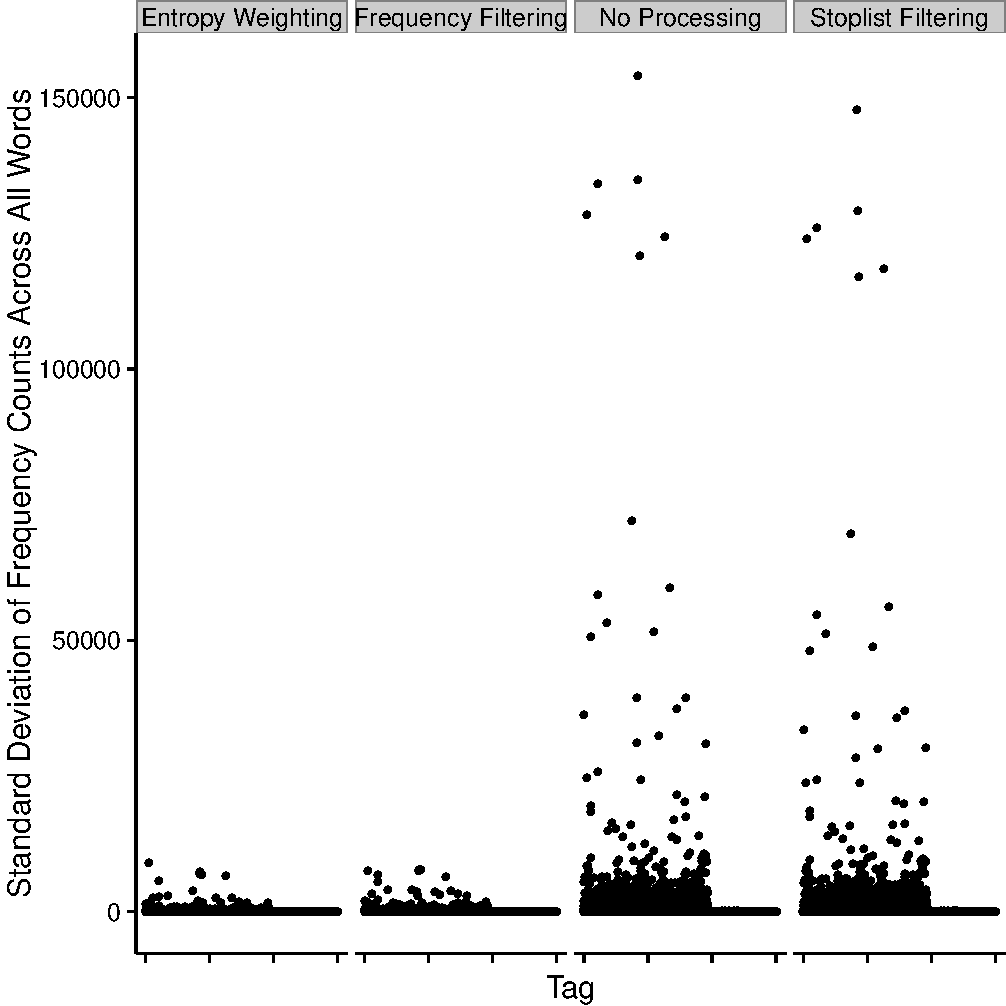
\includegraphics{memMatSO-crop.pdf}}}
  \caption{
    Variance in observation counts of words for each tag for StackOverflow.
    Plots are shown for the four different methods for handling stop words.
    Each plot contains the standard deviation of the total counts for each word in context as a function of hashtag.
    High values mean that there are context words for a hashtag that have a high number of counts relative to the counts for all other context words for that hashtag.
  }
  \label{figContextCutoffSO}
\end{figure}

\begin{figure}[!htbp]
  \scalebox{.6}{\resizebox{\linewidth}{!}{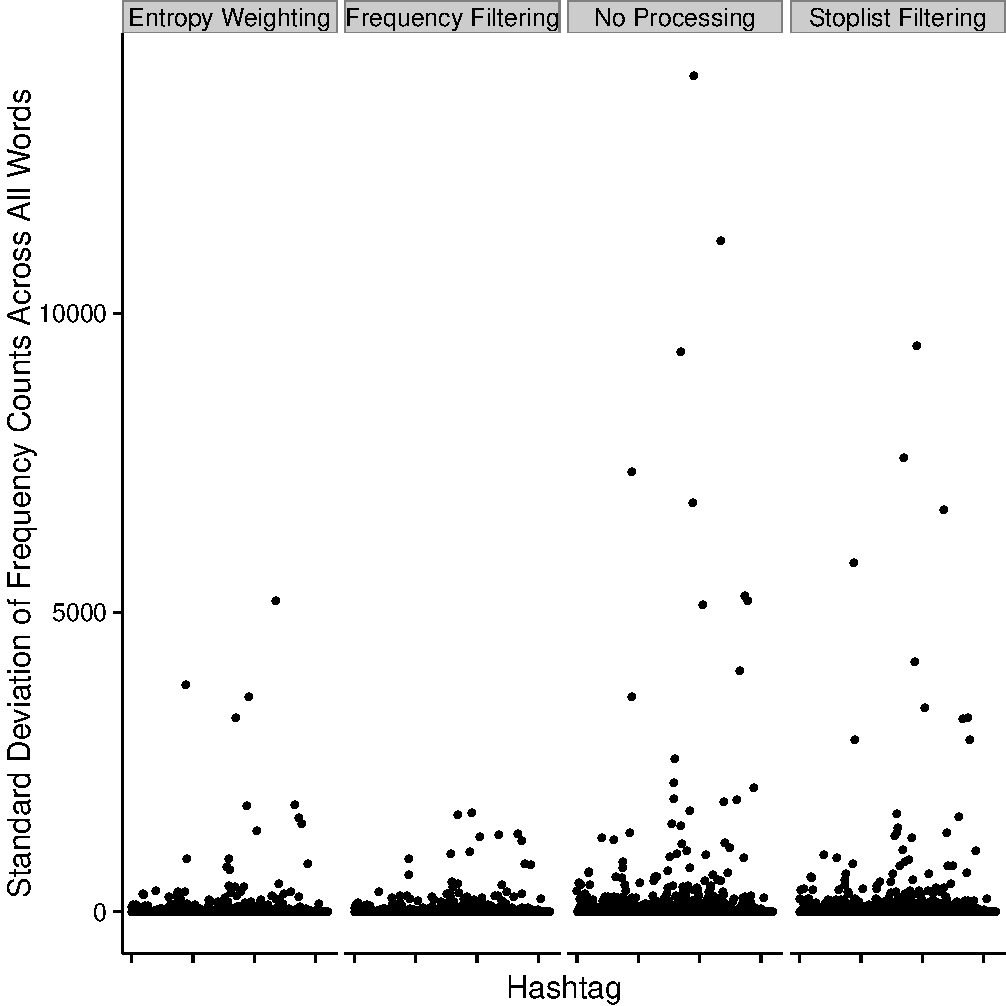
\includegraphics{memMatT-crop.pdf}}}
  \caption{
    Variance in observation counts of words for each tag for Twitter.
  }
  \label{figContextCutoffT}
\end{figure}

The no processing plot shows the size of the spikes when high-frequency words are not removed.
The entropy plot shows how the size decreases by more than an order of magnitude after the entropy weighting measure is used (compare the difference between the no processing subplot and the entropy subplot).
The cutoff for the frequency plot was chosen such that the plot looks similar to the entropy plot, with spikes around the same size.
The cutoff that produced the frequency plots in Figures \ref{figContextCutoffSO} and \ref{figContextCutoffT} is where a word represents more than \num{.04}\% of total occurrences in the dataset.
This may or may not be equal to the value for \textcite{Sahlgren2008}, since that number was expressed in total observations (not as a percentage), and the total number of words in the dataset was not given.

\subsubsection{Results for the Random Permutation Model}

Plots for the three methods of handling stop words for the random permutation model on the StackOverflow dataset are shown in Figure \ref{figContextStopRPSO}.
In the plot, if the model name includes ``full'' then all model components are included.
When the model components are enumerated, then at least one of the components is left out.
So, for example, the ``standard prior model relaxed across posts'' means that only the prior model component was used when determining activation. 
As another example, ``RP only title with freq'' means that only the title context component was used, and that stop words were handled using the frequency filtering technique.

\begin{figure}[!htbp]
  \scalebox{.8}{\resizebox{\linewidth}{!}{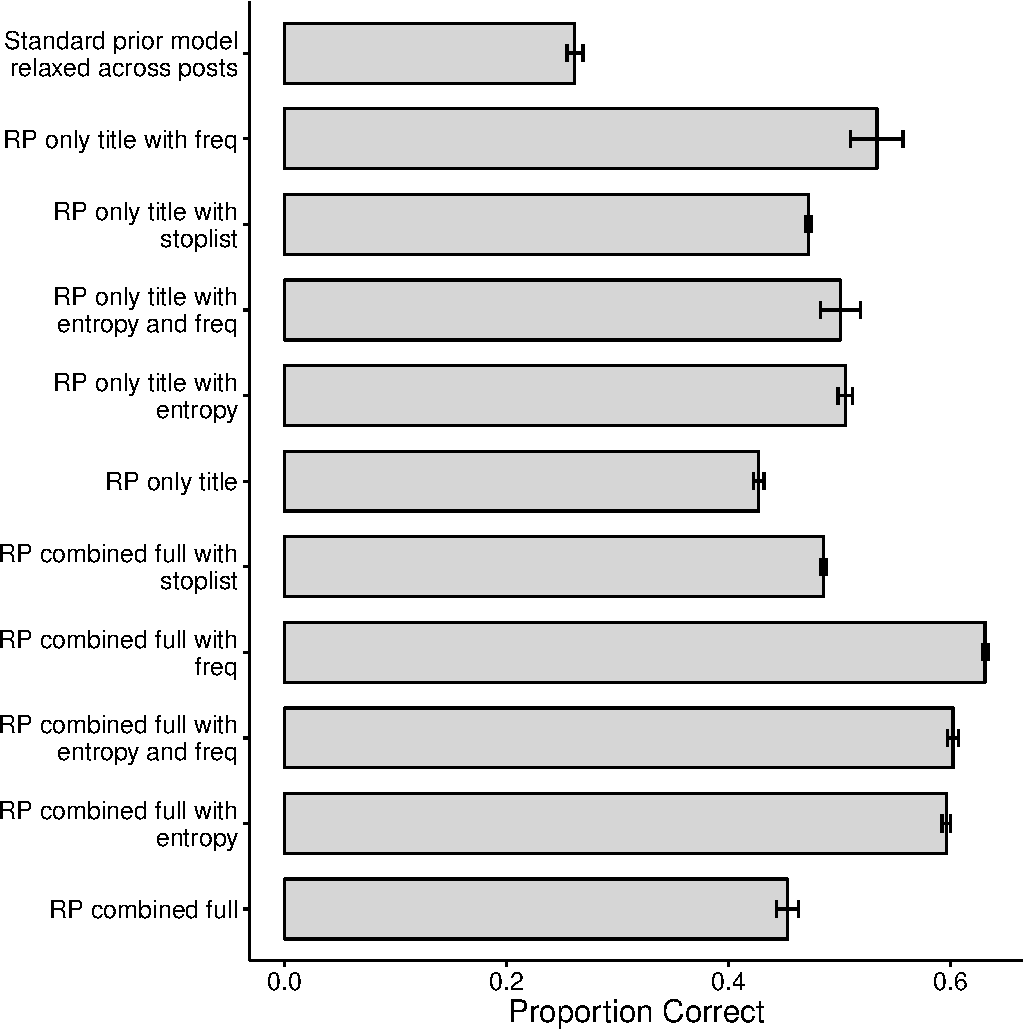
\includegraphics{compareMeanDV-acc-allWeightingsSOPerm-crop.pdf}}}
  \caption{
    Stop-word techniques for the random permutation model for StackOverflow.
    The five methods for handling stop words are shown both for the title model component in isolation and the full model.
    ``Stoplist'', ``freq'', ``entropy'' are the stoplist removal method, removal based on frequency count, and weighting based entropy metric.
}
  \label{figContextStopRPSO}
\end{figure}

The results show that model accuracy improves if stop words are handled in any of the three ways (predefined stoplist filtering, entropy weighting, and frequency filtering).
Using a predefined stoplist makes the smallest improvement (\numNoZero{.45} to \numNoZero{.49}), while the entropy (\numNoZero{.60}) and frequency (\numNoZero{.63}) techniques improve performance the most,
and frequency shows a slight edge over entropy.
However, using the frequency-weighting technique produces more noise in accuracy measurements compared to the other techniques, at least when tested on words in the title of StackOverflow posts.

The three stop word techniques were then tested for the random permutation model on the Twitter dataset, and the results are depicted in Figure \ref{figContextStopRPT}.
For the random permutation model for Twitter, the entropy weighting technique is the best method for handling stop words (\numNoZero{.25} to \numNoZero{.26}).
Removing stop-words based on a predetermined list actually decreases accuracy (\numNoZero{.25} to \numNoZero{.23}), and using data-driven frequency filtering has only a small to no effect (\numNoZero{.25} to \numNoZero{.25}).

\begin{figure}[!htbp]
  \scalebox{.8}{\resizebox{\linewidth}{!}{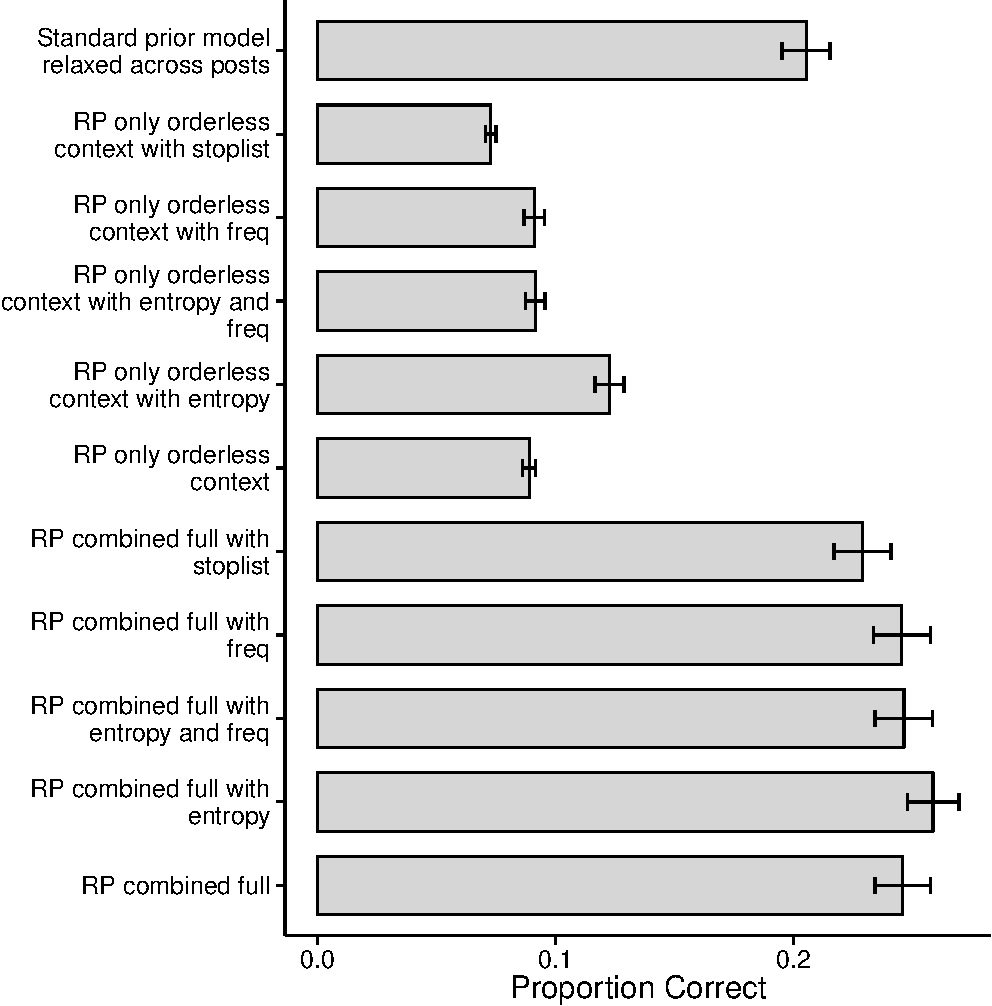
\includegraphics{compareMeanDV-acc-allWeightingsTPerm-crop.pdf}}}
  \caption{
  Stop-word techniques for the random permutation model for Twitter.
  The five methods for handling stop words are shown both for the context model component (i.e., no prior term) and the full model.
}
  \label{figContextStopRPT}
\end{figure}

\subsubsection{Results for the Bayesian Model}

Since accuracy measurements when using a predetermined list to remove stop words for the random permutation model were much worse than the frequency and entropy methods, this method was not examined for the Bayesian model.
The results for the frequency and entropy techniques for the Bayesian model on the StackOverflow dataset are depicted in Figure \ref{figContextStopBSO}.

\begin{figure}[!htbp]
  \scalebox{.8}{\resizebox{\linewidth}{!}{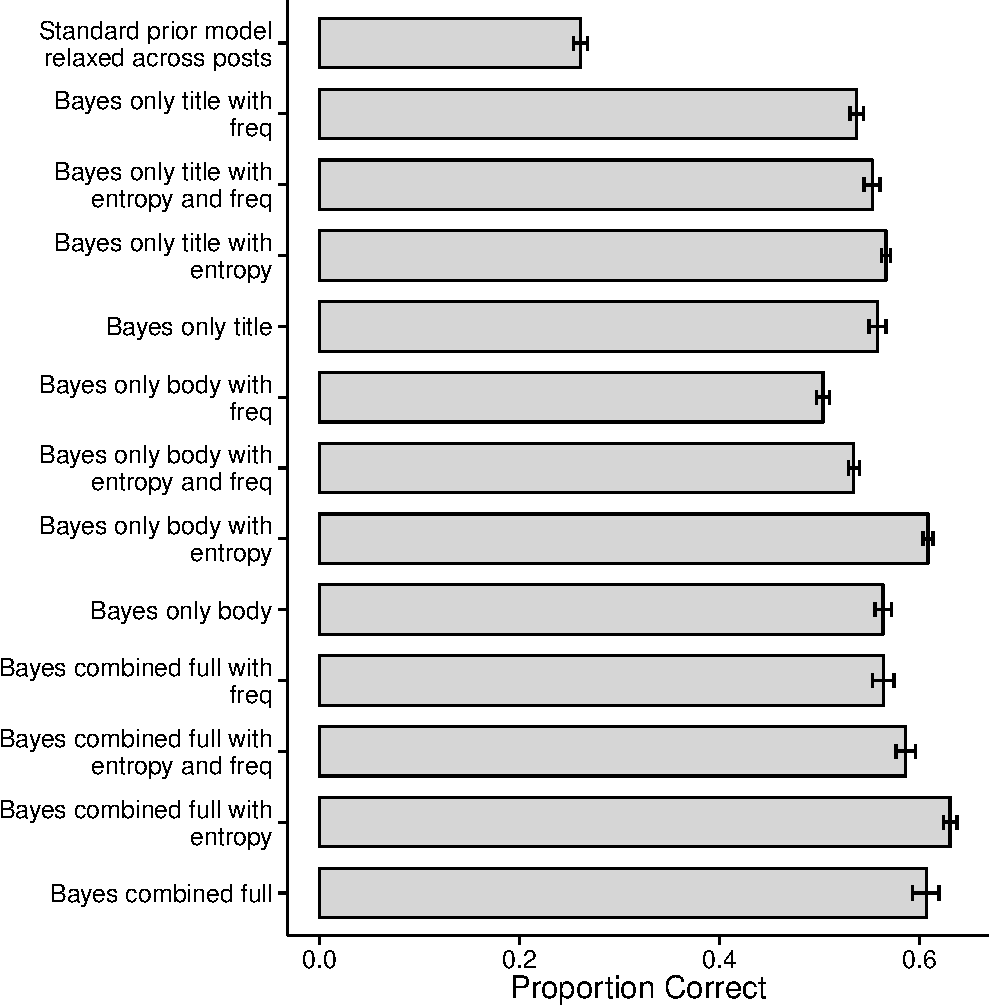
\includegraphics{compareMeanDV-acc-allWeightingsSOSji-crop.pdf}}}
  \caption{Stop-word techniques for the Bayesian model for StackOverflow}
  \label{figContextStopBSO}
\end{figure}

The results show that entropy weighting produces the most accurate results (\numNoZero{.61} to \numNoZero{.63}).
Also, accuracy actually decreases when using frequency filtering (compared to no filtering) (\numNoZero{.61} to \numNoZero{.56}) for the Bayesian model.
So entropy weighting is the clear winner in this case.

Similar results are found when the Bayesian model is tested on the Twitter dataset.
Figure \ref{figContextStopBT} shows that entropy weighting is again the best performer (\numNoZero{.29} to \numNoZero{.32}),
and frequency filtering decreases performance relative to no filtering (\numNoZero{.29} to \numNoZero{.28}).

\begin{figure}[!htbp]
  \scalebox{.8}{\resizebox{\linewidth}{!}{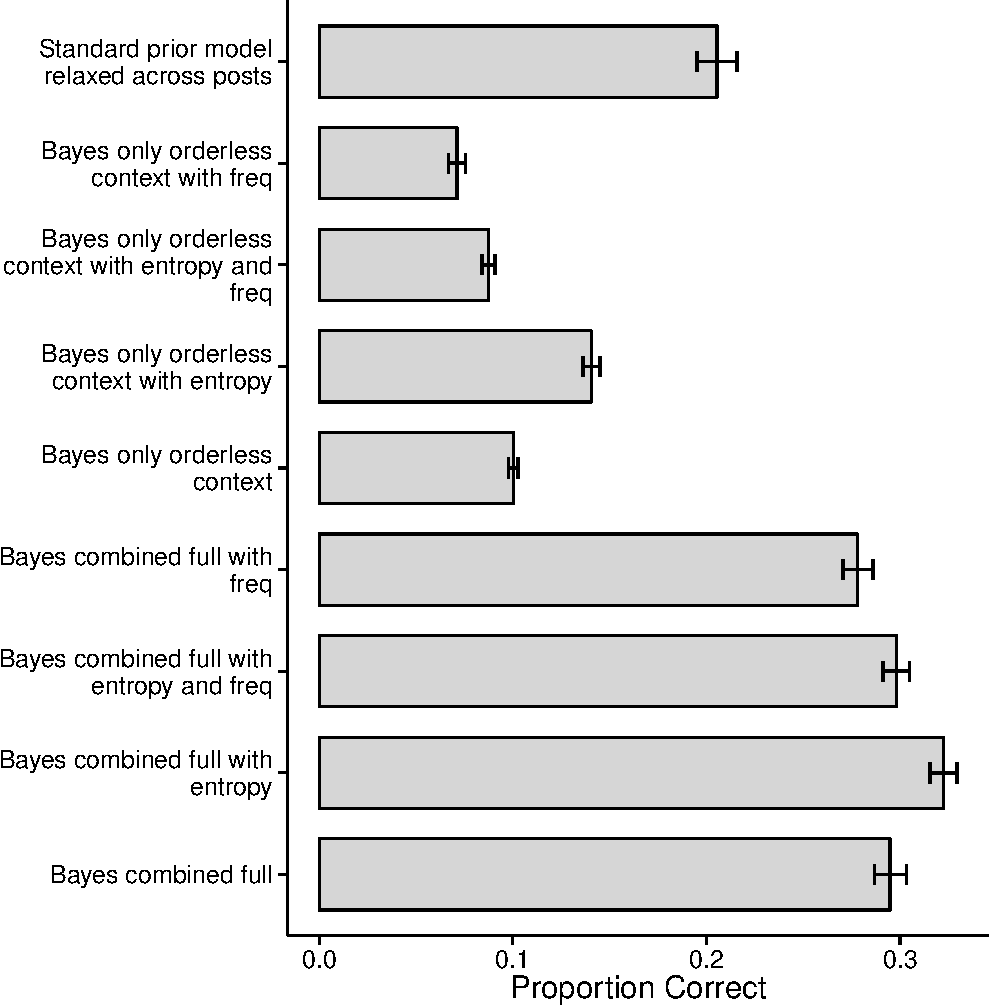
\includegraphics{compareMeanDV-acc-allWeightingsTSji-crop.pdf}}}
  \caption{Stop-word techniques for the Bayesian model for Twitter}
  \label{figContextStopBT}
\end{figure}

\subsubsection{Discussion}

One result that should not be overlooked is how poorly using a predetermined stoplist performed when compared to the two data-driven frequency and entropy approaches.
This is most likely because the StackOverflow and Twitter datasets are large and contain high-frequency words that are domain specific (e.g., emoticons) and are not included in the predetermined list.
This shows that data-driven techniques to identify stop words can be much more effective than using a predetermined list.

Another interesting result is how the Bayesian model actually performed worse when stop words were removed based on frequency compared to no stop word removal.
This was not the case for the random permutation model in this study, was not the case when \textcite{Sahlgren2008} used frequency filtering on the random permutation model,
and is most likely never the case for the random permutation model.
Model accuracy most likely decreases for the Bayesian model because this model already has a normalization component built in that the random permutation model does not have.
When computing activation for the random permutation model, the correlation is calculated directly on a matrix of counts of co-occurrences for words and tags.
For the Bayesian model this count matrix is converted to a log-odds ($S_{ji}$) matrix,
where both the number of observations for the word and the tag are normalized when computing the value for each cell (see the $S_{ji}$ computation in Table \ref{tabModACTRModel}).
So it is likely the case that a form of frequency attenuation is already built into the Bayesian model.
Therefore, adding a frequency filter on top of this does nothing to improve accuracy and only removes predictive information.

\textcite{Stanley2013} found that the entropy-weighting technique to attenuate stop words for the Bayesian model significantly improved model accuracy.
The same effect is found for the StackOverflow and Twitter datasets in this study.
Further, when this entropy-weighting technique is compared directly to the more common frequency-filtering technique, weighting by entropy produces more accurate results.
This was clearly the case for the Bayesian model.
Both frequency and entropy techniques performed equally for the random permutation model.
However, since the entropy-weighting technique is parameter free and does not require a cutoff to tune, it is also a better choice for the random permutation model for these datasets.

The effect sizes when comparing no stop-word removal technique to either the entropy or frequency techniques are quite large.
This shows the importance of correctly identifying and handling stop words when building co-occurrence matrices for large-scale natural language datasets.
For further research, it may be worthwhile to explore an even larger range of stop-word handling techniques,
since model accuracy seems to be quite sensitive to the specific method used. 
However, one conclusion that can be made from this research is that the entropy-weighting method is a contender, and should be considered much more often than it has been previously.

\subsection{Corpus Size}

The number of documents used to build the co-occurrence matrix has been shown to influence model accuracy \parencite{Sahlgren2008}, so this was the second architectural concern that was examined.
The default number of documents used to build the co-occurrence matrix was \num{1000000} for StackOverflow and \num{3000000} for Twitter.
In order to see how accuracy changed as function of corpus size, 
co-occurrence matrices for a range of smaller corpus sizes were built.
Both the random permutation and Bayesian models were tested on all corpus sizes.

\subsubsection{Method}

For StackOverflow, the following number of posts were used to build separate co-occurrence matrices: \num{1000}, \num{10000}, \num{100000}, and the default \num{1000000}.
For Twitter, these matrix sizes were tested alongside the default \num{3000000}.
All runs from the four Twitter popular-hashtags datasets and the randomly-sampled StackOverflow dataset were used to test model accuracy.

\subsubsection{Results for StackOverflow}

Model accuracy as a function of co-occurrence matrix size for StackOverflow is depicted in Figure \ref{figContextDocumentSizeSO}.
Accuracy improves for both the Bayesian and random permutation models as the size of the documents used to generate the co-occurrence matrix increases.
However, model accuracy using the entropy weighting technique plateaus and slightly decreases for the largest corpus size for the random permutation model, while the frequency technique only begins to plateau. 
The Bayesian model does not plateau and accuracy continues to improve as corpus size increases.

\begin{figure}[!htbp]
  \scalebox{.8}{\resizebox{\linewidth}{!}{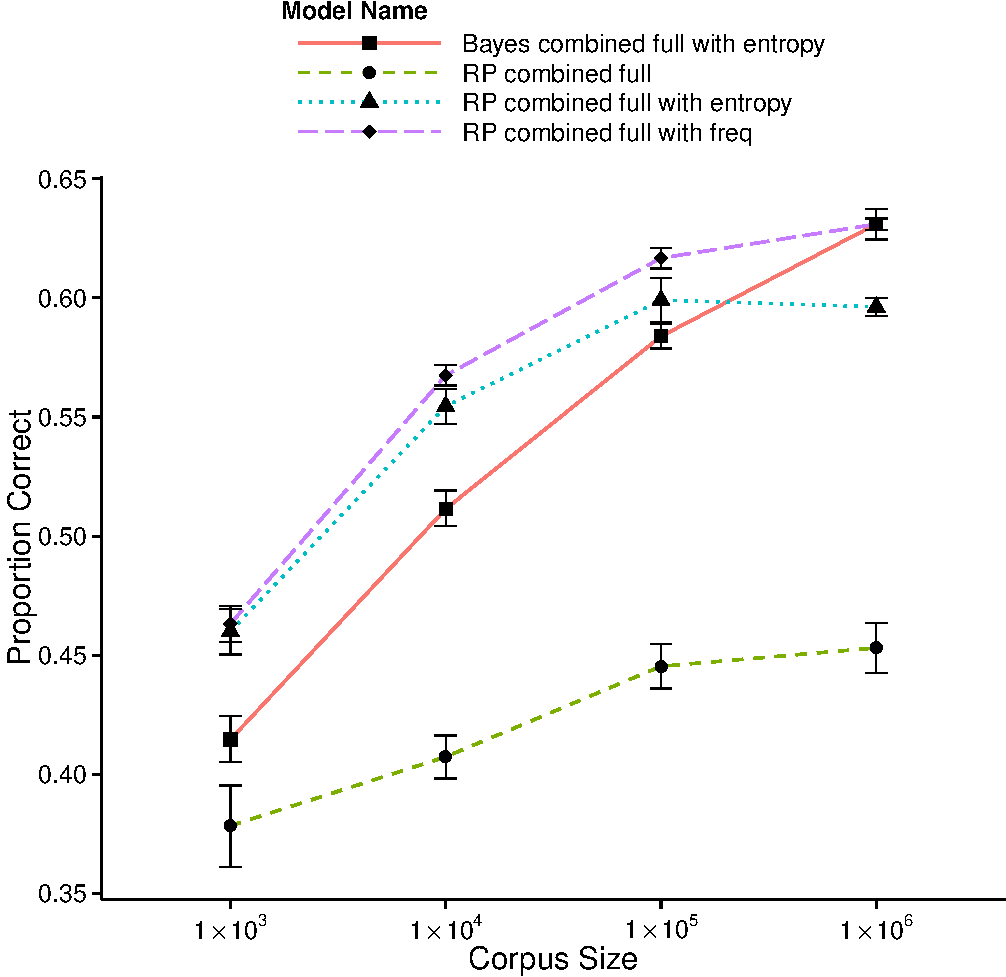
\includegraphics{compareMeanDV-acc-freqVsEntropyBySizeSO-crop.pdf}}}
  \caption{
    Effect of size of co-occurrence matrix for StackOverflow.
    Error bars represent the 95\% bootstrapped confidence interval for the mean model accuracy across all runs in dataset.
  }
  \label{figContextDocumentSizeSO}
\end{figure}

\subsubsection{Discussion}

It is likely that the random permutation model is starting to saturate when entropy weighting is used for the largest corpus size for StackOverflow.
Saturation happens when certain words co-occur with a tag much more often than all of the other words.
This introduces range effects when the correlation is computed, which ends up driving all of the correlations near one, and consequently decreases discrimination and accuracy.
Saturation happens when entropy weighting is used because the non-predictive words are only attenuated and not removed, and this attenuation is not enough to overcome the range effects that grow with corpus size.

However, the effect of saturation is small compared to the large effect from using either frequency filtering or entropy weighting to handle the stop words.
The Bayesian model does not saturate when using entropy weighting because each cell in the co-occurrence matrix is normalized by word frequency and tag frequency.

\subsubsection{Results for Twitter}

The overall trend of increasing accuracy with corpus size is present for Twitter as well.
Both entropy weighting and frequency filtering in Figure \ref{figContextDocumentSizeT} plateau for the random permutation model with increasing corpus size.
Once again, the Bayesian model continues to improve with corpus size.

\begin{figure}[!htbp]
  \scalebox{.8}{\resizebox{\linewidth}{!}{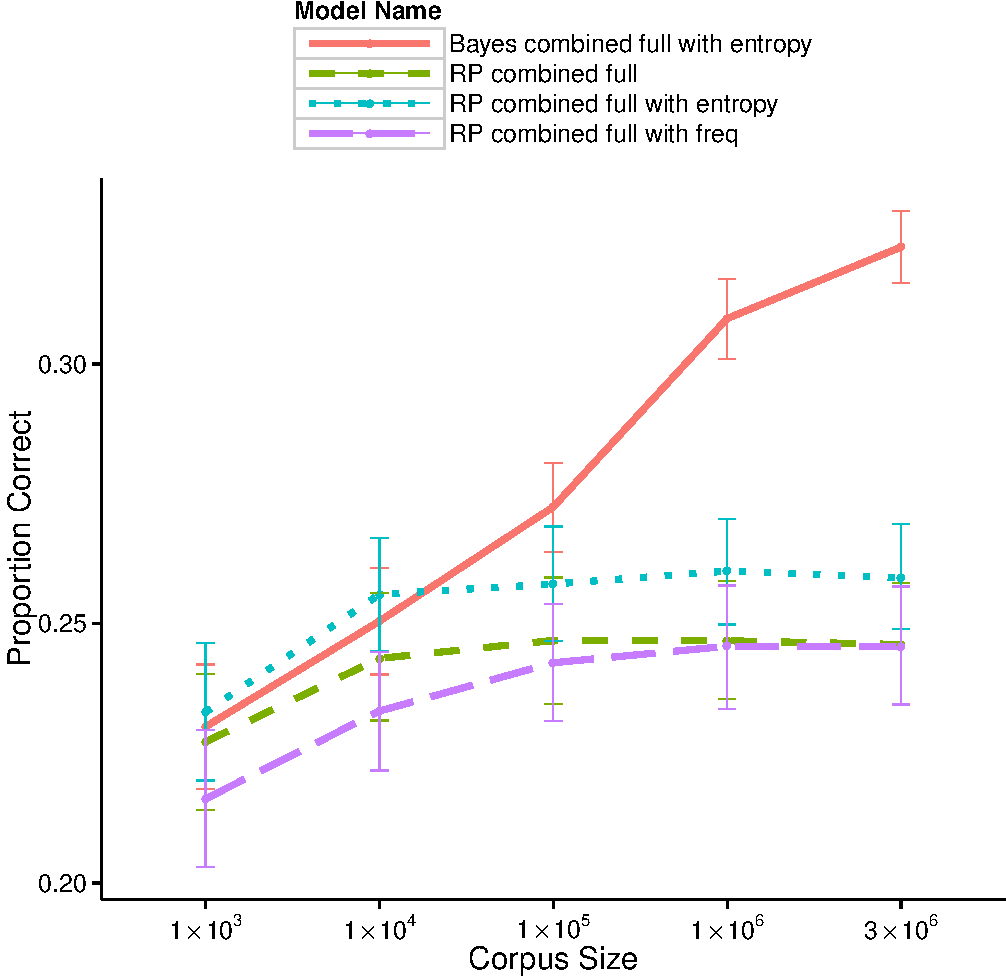
\includegraphics{compareMeanDV-acc-freqVsEntropyBySizeT-crop.pdf}}}
  \caption{
    Effect of size of co-occurrence matrix for Twitter.
    Error bars represent the 95\% bootstrapped confidence interval for the mean.
  }
  \label{figContextDocumentSizeT}
\end{figure}

\subsubsection{Discussion}

It is interesting to compare model accuracy between the Bayesian and random permutation model at the smallest and largest corpus sizes for both StackOverflow and Twitter.
At smaller corpus sizes, the random permutation model outperforms the Bayesian model (slightly for Twitter, dramatically for StackOverflow), and this performance difference deteriorates as corpus size increases.
In other words, the Bayesian model needs larger co-occurrence matrices than the random permutation model to work properly.
As the size of the dataset increases, the compression may start to lose crucial information, and the uncompressed Bayesian model should be used.
As the size of the dataset decreases, the noise and crosstalk introduced by the compression for the random permutation model is actually beneficial, and the compressed random permutation model should be used. 
This noise is beneficial because it helps soften spurious $S_{ji}$ values when the counts for each individual cell in the co-occurrence matrix are still volatile, which happens at smaller corpus sizes.

This result has important implications.
The corpus size is rarely chosen, and more likely constrained by the number of documents in the dataset being studied.
If that dataset is relatively small, it may be better to use the compressed random permutation model than the Bayesian model, and vice-versa if the dataset is large.

However, corpus size is not the only factor that determines whether the Bayesian model or random permutation model will perform better.
For example, the corpus size where the Bayesian model begins to outperform the random permutation model is quite different for StackOverflow and Twitter.
This is because the number of observations used to generate the co-occurrence matrix is a function of four components:
corpus size, number of words in each document, total number of unique tags, and number of tags used per document.

The transition point where accuracy for the Bayesian model outperformed the random permutation model was much higher for StackOverflow than Twitter.
This is most likely because StackOverflow has almost \num{100} times more unique tags than the Twitter popular-hashtags dataset.
The number of words in a StackOverflow post is also much higher than Twitter, which should have lowered the transition point.
However, the effect of words in a post must be less than the effect of number of unique tags, as the transition point was still much higher for StackOverflow given that it should have lowered due to post size.

The compressed random permutation model should perform better with smaller corpus sizes, less words per document, more unique tags, and fewer number of tags per post.
However, since there are so many factors that determine whether the Bayesian or random permutation model will perform better,
and only two different datasets were examined in this research,
it is difficult to make any specific recommendations as far as exact transition cut points (e.g., corpus size, words per document) where either the Bayesian or random permutation model should be used.
Also, it is likely that the specific domain being studied interacts with the factors already mentioned to determine which model is better for that domain.
Nevertheless, if a researcher is working in a domain with limited data (e.g., small corpus size, large tag space) that produces a sparse co-occurrence matrix,
then it may be worthwhile to experiment with using a compressed random permutation model instead of the full Bayesian model.

\subsection{Combining Prior and Context}

The activation value for the context component of the vector-based model is a correlation, ranging from zero to one.
This is not a log-odds value.
For the previous results, prior and context for the random permutation model were combined by simply adding the terms.
However, this means that ACT-R's prior base-level learning component (which is a log-odds value) is added to a correlation value, which may not be mathematically appropriate.
As a fourth architectural concern, another method to combine the prior and context components for the random-permutation model was explored.

\subsubsection{Method}

For a given retrieval, the random permutation model returns a set of activations that are correlation values for each of the tags.
Instead of simply adding this correlation value to the prior model term, it may be more appropriate to convert the correlation value to a log-odds value first, and then add this context term to the log-odds prior term.
So a method was created to convert a distribution of correlations to a distribution of log-odds values.
To do this, the one-tailed cumulative distribution function value for each correlation in the distribution was computed.
That probability was then converted to a log-odds value in the usual way. 

This technique has a few advantages: 
It is simple and computationally cheap.
Also, it behaves properly at specific points in the distribution.
For example, if the conversion is performed on the mean correlation value in the set, the result is a log-odds value of zero.
This makes sense given that log odds can be interpreted as the amount of odds information (positive or negative) that should be adjusted to the prior log odds, given that new piece of information.
Since the mean correlation value contains no information regarding if it is better or worse than the other correlation values, it is appropriate to assign this correlation value a zero log-odds adjustment value.

The log-odds transformation technique was tested for the random permutation model on the Twitter popular-hashtags and StackOverflow randomly-sampled datasets.

\subsubsection{Results}

Model accuracy results after using the log-odds transformation are depicted in Figures \ref{figContextLogoddsSO} and \ref{figContextLogoddsT}.
Using the log-odds transformation technique has a small effect on model accuracy for StackOverflow (\numNoZero{.45} to \numNoZero{.47}) and minimal to no effect on Twitter (\numNoZero{.25} to \numNoZero{.25}).
When the technique is used and accuracy is examined for a model with only a single predictor, the transformation does not change accuracy.
When predictors are combined and the full model is examined, the transformation is in the direction of slightly increasing accuracy, at least for the StackOverflow dataset.
However, any improvement when using the transformation is minimal.

\begin{figure}[!htbp]
  \scalebox{.6}{\resizebox{\linewidth}{!}{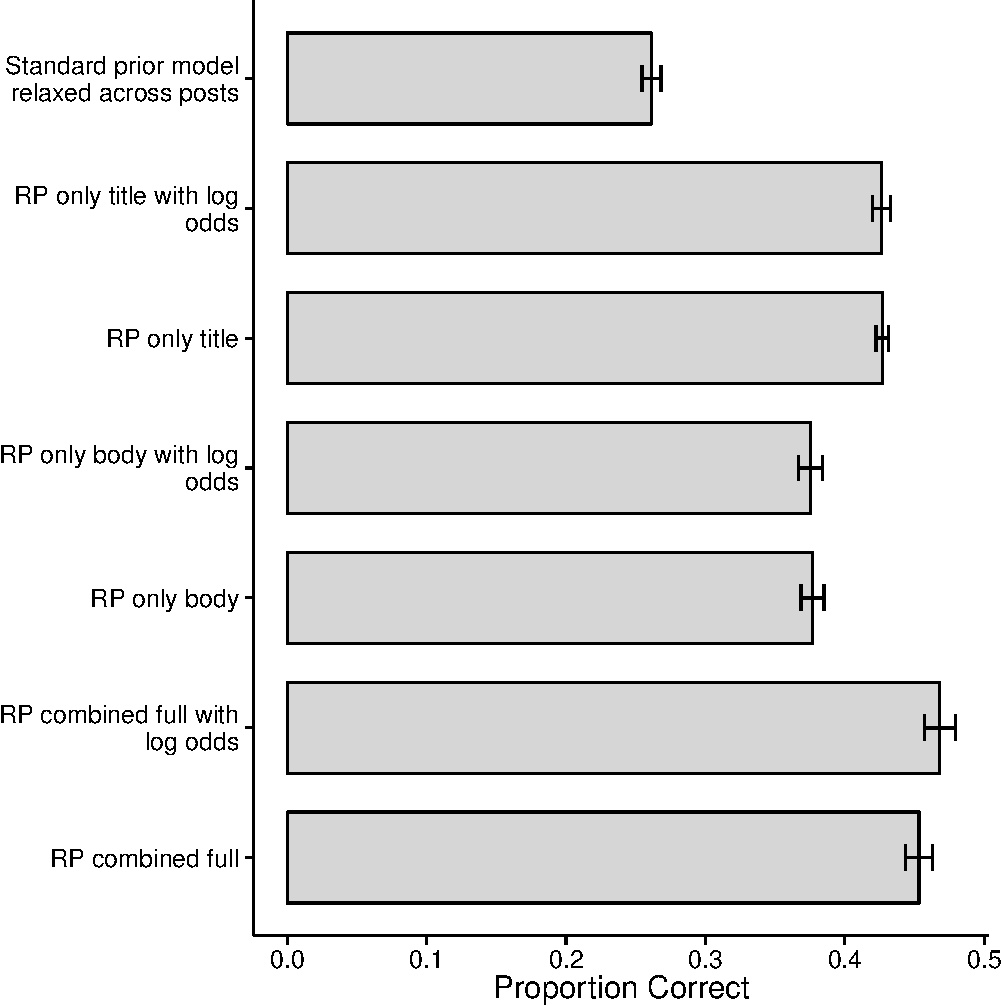
\includegraphics{compareMeanDV-acc-logoddsSO-crop.pdf}}}
  \caption{Random permutation model accuracy when using log-odds transformation on context for StackOverflow}
  \label{figContextLogoddsSO}
\end{figure}

\begin{figure}[!htbp]
  \scalebox{.6}{\resizebox{\linewidth}{!}{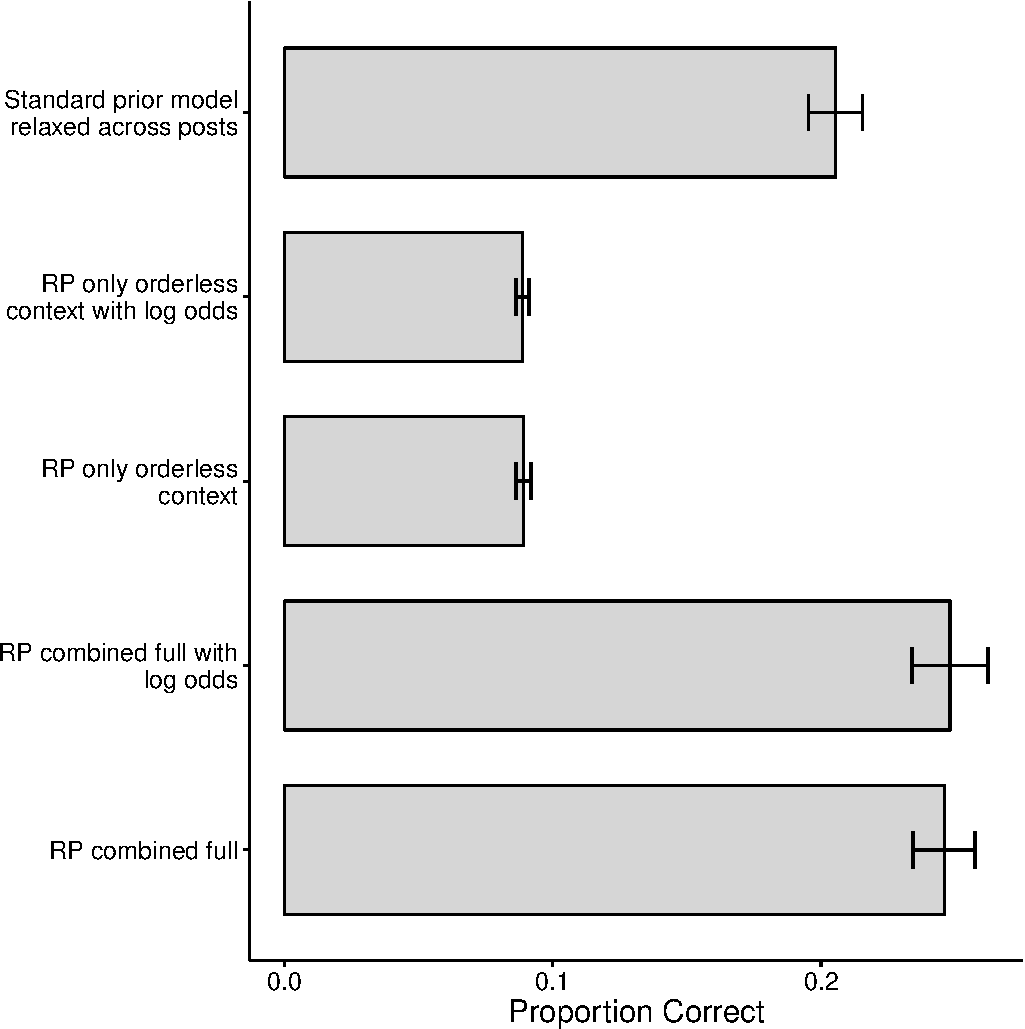
\includegraphics{compareMeanDV-acc-logoddsT-crop.pdf}}}
  \caption{Random permutation model accuracy when using log-odds transformation on context for Twitter}
  \label{figContextLogoddsT}
\end{figure}

\subsubsection{Discussion}

Vector-based models such as the random permutation model \parencite{Sahlgren2008} have included only a context component in the past (i.e., no prior component).
When the prior component is included for the random permutation model, accuracy improves significantly (compare accuracy for full models to context models in Figures \ref{figContextLogoddsSO} and \ref{figContextLogoddsT}).
However, it is somewhat surprising that it does not matter much how the context and prior terms are added for the random permutation model.
Model performance is similar when the context component used for the model is based on a correlation compared to a log-odds value.

There may be a slight edge in increased accuracy when a log-odds transformation is used for the StackOverflow dataset.
However, that result is not statistically reliable for the sample size used in this analysis (confidence intervals overlap in Figure \ref{figContextLogoddsSO}),
and even if present the overall change in accuracy is small (\numNoZero{.45} to \numNoZero{.47}).
Nonetheless, it does seem appropriate to convert the context to a log-odds adjustment value when context is added as an additional term to the random permutation model.
Since performance does not decrease when the transformation is made, may slightly increase,
and leads to a more natural interpretation of each model term as a log-odds value, it is reasonable to include this step for the random permutation model.
Future research could explore additional methods to properly combine the terms.

\subsection{Word Order}

As a final architectural concern, vector-based models with and without word order were tested to examine the effect of word order on model accuracy.
Vector-based models like the random permutation model can easily incorporate word order when making predictions.
This is one of their primary strengths that has been discussed \parencites{Jones2007, Sahlgren2008}.
In order to thoroughly test the impact of adding word order into the model, various methods for incorporating word order were tested on the StackOverflow and Twitter datasets.

\subsubsection{Method}

Three different methods for incorporating word order in the random permutation model were tested:
taking just the sign of the word's position relative to the tag (direction method), using the position (standard method), and using the position but only including words that were used near the tag (window method).
For the standard method, all words and their respective position are used to build the representation.
For the direction method, essentially two representations are created: all co-occurrences with words to the left of the tag, and all co-occurrences with words to the right of the tag.
The window method is similar to the standard method, where each word's relative position is maintained, but it only includes words near the tag to build the representation.
\textcite{Sahlgren2008} tested similar methods, and found that accuracy was highest when a narrow window was used for the window method (only including words at most two positions to the left and right of the tag).
The same $+2$ $-2$ range was used to test the window method on the Twitter dataset.

Only the Twitter dataset was tested, since the StackOverflow dataset contains no word order information between words in the title and body of the post and the tags used for the post.
The author chooses tags after filling out the title and body forms in the post, so the tags are never intermixed with words in the post like they are for Twitter.

The same four Twitter popular-hashtags datasets were used for testing.
Both an ordered and orderless context component were created for the random permutation models.
The orderless context component uses the same co-occurrence matrix used by the Bayesian model to create the representation, since the Bayesian model does not contain any order information.
Models were tested that used only one of the three word order methods for the ordered context component, used only the orderless context component, used a combination of the two components, and combined context with prior. 

\subsubsection{Results}

Model accuracy results after incorporating word order into the random permutation model are depicted in Figure \ref{figContextOrder}.
All bar plots that include an order component where ``window'' or ``direction'' is not included in the title use the standard ordering method (no direction or windowing, all position information is included) 
This is the default ordering method used, so the names for these bar plots were kept consistent to the names used in other figures so that comparisons could be made across figures if necessary
(similar to what was done for the default row size for the random permutation model).
Base models that do not use entropy weighting were also included so that effect sizes could be compared between entropy weighting and adding word order information.

\begin{figure}[!htbp]
  \scalebox{.8}{\resizebox{\linewidth}{!}{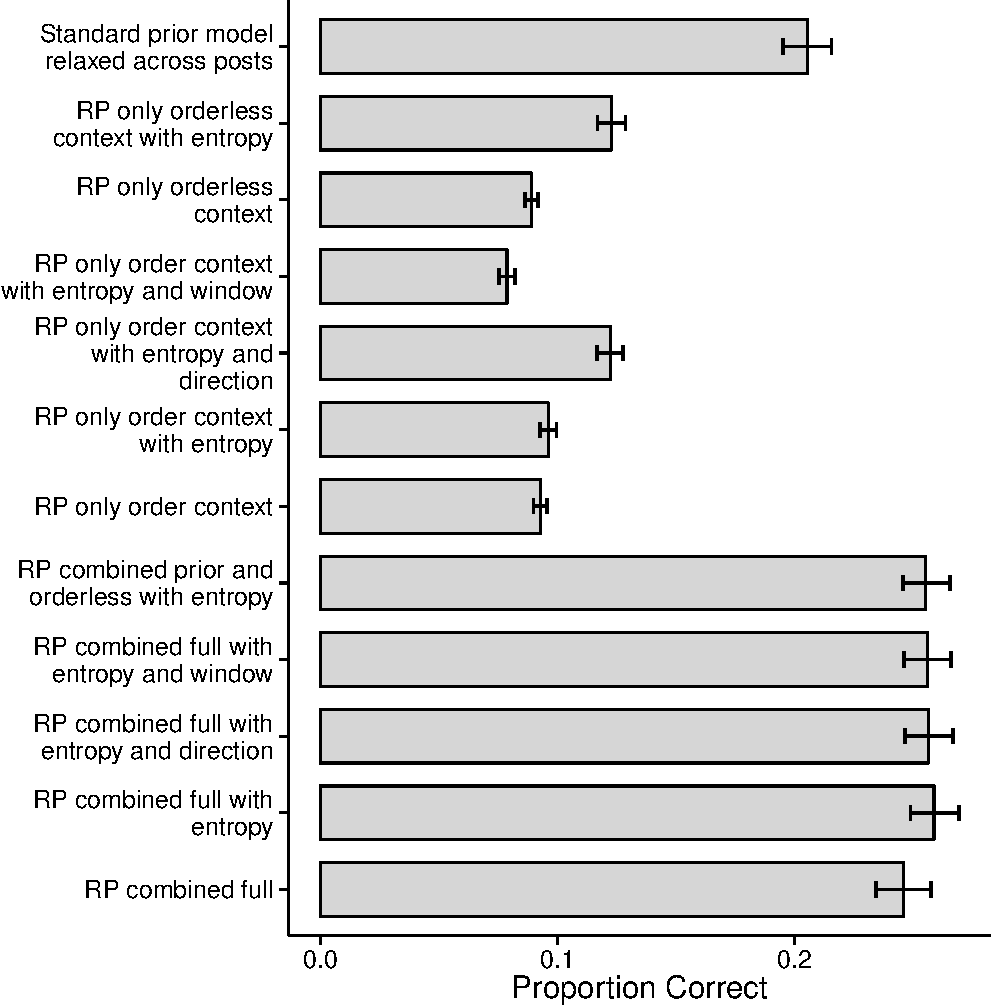
\includegraphics{compareMeanDV-acc-orderT-crop.pdf}}}
  \caption{Model accuracy for various word order methods for the random permutation model for Twitter}
  \label{figContextOrder}
\end{figure}

Looking first at models where no prior is added, the random permutation model using only orderless context performs similar to the model using only order context with direction.
All other order-only models perform worse than the order model using direction and worse than the orderless model.

Full models were also plotted against the model where only the prior and orderless context was included (i.e., no order).
This was to test how much of the variance in model accuracy is shared between the orderless and order models.
The results show that there is little unique variance in the order-only models, so order information contributes little to overall model performance above and beyond what an orderless model contributes.
This can be seen by comparing the two-component model with only prior and orderless context to the three-component model with prior, orderless, and any of the three methods for the order context term.

\subsubsection{Discussion}

This was a surprising result.
One of the main benefits discussed for the random permutation model is that it can easily incorporate word order information into the representation.
But including word order information does not dramatically improve performance. 
For the random permutation model, it is much more important to properly handle low-predictor stop words and include a prior component than it is to include word order information,
at least for the Twitter dataset tested in this study.

The original BEAGLE model \parencite{Jones2007} actually showed only minimal improvement when incorporating word order as well.
In absolute terms, this model only improved by 2 percentage points in accuracy when trained on the TASA and tested on the TOEFL.
\textcite{Sahlgren2008}'s results for word order for the random permutation model are similar.
At a row size of around \num{2000}, model accuracy improves by less than a percentage point when order information is incorporated.

So although incorporating word order into the random permutation model does seem to slightly improve performance,
the strength of the model is more likely to be in how efficiently it can represent the co-occurrence matrix rather than its ability to include word order in the representation.
That is, the strength of the model is in its compressed unordered context component term and not the ordered component, at least for the Twitter dataset studied.

Also, the reason why the directional version of ordering is the best predictor of the three ordered components is most likely because order information does not have a large effect,
so the two representations for words to the left and right of a tag are highly correlated.
This means that this directionally-ordered component is essentially composed of all the co-occurrence observations in the orderless component after being randomly sampled and partitioned into two separate representations.
The co-occurrences in these representations are highly correlated with each other, and highly correlated with the orderless component,
which is why model accuracy is similar for the orderless component and direction ordered component, and why accuracy does not improve when adding the direction ordered component to the orderless component.

\section{Chapter 7: General Discussion}

The general discussion is separated into two parts.
The first section will describe the overall results and reemphasize key findings.
The final section will discuss general theoretical implications of the results and describe future applications and directions. 

\subsection{Overall Results}

Table \ref{tabOverallResults} summarizes model accuracies for full models (all components) on all of the datasets tested in the study.
After modifying the models by adding an entropy weighting mechanism to both models and a prior term to the random permutation model,
accuracy for the compressed random permutation model was nearly equal to the Bayesian model.
The largest difference between the two models was on the Twitter popular-hashtags dataset (7 percent).
Both models performed nearly equal for the StackOverflow datasets tested,
and both models were much more accurate when tested on StackOverflow compared to Twitter.

\begin{table}[!ht]
  \caption{
    Summary of accuracy for each model and dataset.
    The Bayesian model includes entropy weighting for the context words,
    the RP model includes entropy weighting and log odds transformation when combining the context and prior components.
    Both models use a user-customized co-occurrence matrix for the Twitter popular-users dataset, since a global co-occurrence
    matrix is not available for this dataset.
  }
  \label{tabOverallResults}
  {\tabulinesep=1.2mm
    \begin{tabu}{llll}
      \hline
	Site 		& Dataset		& Model						& Accuracy \\
	\hline
	StackOverflow	& popular-users		& Bayesian with entropy				& \numNoZero{.63} \\
			& 			& RP with entropy and log odds 			& \numNoZero{.58} \\
			& randomly-sampled	& Bayesian with entropy 			& \numNoZero{.63} \\
			& 			& RP with entropy and log odds			& \numNoZero{.63} \\
	Twitter		& popular-users		& Bayesian with entropy and user sji		& \numNoZero{.39} \\
			& 			& RP with entropy, log odds, and user sji	& \numNoZero{.39} \\
			& popular-hashtags	& Bayesian with entropy				& \numNoZero{.32} \\
			& 			& RP with entropy and log odds			& \numNoZero{.25} \\
	\hline
    \end{tabu}
  }
\end{table}

Overall, both the random permutation and Bayesian declarative memory models fit the observed tagging behavior in StackOverflow and Twitter relatively well.
The fits for StackOverflow in particular are quite high, especially given the large tag space on the site.
These results provide support for the idea that choosing a hashtag when composing a tweet and tagging a StackOverflow post is akin to a declarative memory retrieval process.
However, both models were not 100 percent accurate, and the amount of variance left to predict was much larger than what would be observed if retrieval noise was included in the model.
So it is most likely the case that the task is not done solely with declarative memory processes.

\textcite{Anderson1991} also looked at similar tagging tasks with large datasets when deriving the prior component of the declarative memory theory.
\citeauthor{Anderson1991} examined, for example, the frequency of word choice over time used for the title of articles for the New York Times,
and used the results to derive the power law equation for the prior term in the declarative memory model.
ACT-R's declarative memory theory claims that the system has evolved to make predictions that closely match the statistical structure of the environment.
Using a power-law equation to model future tag use based on past tag use is a reasonable statistical approach to the problem.
It is also the case that this same equation is an accurate model for the prior component of declarative memory, as was shown by \citeauthor{Anderson1991} in the original derivation, 
and as is supported in the results from this study.

\subsubsection{Representation}

Given that the storage space required to represent the co-occurrences for the random permutation model is dramatically smaller than the uncompressed Bayesian model,
and that the compression is lossy and essentially random (i.e., no SVD),
it is quite interesting that the random permutation model performs nearly as well as the full Bayesian model for this task.

These results pose an interesting and important fundamental question about declarative memory:
How, precisely, is the neural system configured to represent co-occurrences for declarative memory?
Since at the behavioral level both models perform similarly, it is possible that the neural system is using either representation to store co-occurrences.
Vector-based models are simple enough that they can easily be implemented in a neural network.
Perhaps a form of vector-based compressed storage is being used at the neural level,
since it can be implemented in neurons and is an efficient way for the machinery to generate predictions that closely match the statistical structure of the environment
(i.e., that closely match the uncompressed Bayesian representation).

As neural imaging systems improve, this question of neural representation can be best answered by looking directly at the neural activity.
However, there are possible behavioral studies that could be done to provide evidence that may favor one representation over the other:
The largest differences between the Bayesian and vector-based models happen with small numbers of co-occurrence observations.
The vector-based model begins to generate more accurate predictions sooner than the Bayesian models,
since the noise introduced from the compression helps smooth out activation values until a larger number of co-occurrences are observed and the co-occurrence values stabilize.
For a behavioral study, novel words could be introduced alongside a corpus of known words, and the participant could be asked to make retrievals of the novel words and known words as more novel words are introduced.
Both models would make different predictions about the rate at which activation values for the novel words stabilize relative to the known words, and such make different predictions about retrieval error rates over time.
Learning a new language might be a domain where large amounts of these sorts of retrievals could be collected.
For instance, the online site Duolingo might contain enough collective data about language learning and word translation to better tease apart the two context models.

\subsubsection{Compression}

Also, the relatively strong performance of the random permutation model is not due to the model's ability to represent word order.
Performance is similar for the random permutation and Bayesian models when the co-occurrence matrix for both models is the same, and not based on word order.
Performance also does not improve by much when word order is added as the last predictor in the random permutation model.
The random permutation model seems to work so well primarily due to the way that the full co-occurrence representation is compressed.

As previously noted, compression for the random permutation model is essentially random.
That is, no SVD is done to identify the most predictive components,
so the compressed representation used by the random permutation model does not contain nearly as much of the variance from the original co-occurrence matrix that it could have.
However, performing a full SVD on a co-occurrence matrix as large as the ones generated for StackOverflow and Twitter is computationally infeasible.
Also, when deriving the LSA approach, \textcite{Landauer1997} explicitly state that they make no claims that the brain is computing an SVD at the neural level;
only that the neural machinery is set up such that the representation makes predictions that are similar to what would have been generated if the matrix decomposition for an SVD would have been computed.
Perhaps the randomly-compressed representation used for the random permutation model is the way in which the brain tries to efficiently achieve the full LSA- and SVD-like approach that \citeauthor{Landauer1997} propose.

\subsubsection{Attentional Weight}

The Bayesian declarative memory model for ACT-R has an attentional weight term $W_{j}$ that can be used to attenuate or remove stop words.
The random permutation model was also easily modified to have an attentional weight term by attenuating each word's set of ones and negative ones values by that word's attentional weight.
Both a method for stop-word removal (frequency filtering) and stop-word attenuating (entropy weighting) performed well for both models.
Also, using a proper method for handling the low-predictor words produced some of the largest improvements in model accuracy compared to the other explorations
(e.g., compared to word order, properly adding terms, compression amount for random permutation representation).
Since the ACT-R declarative memory theory already has a component for attentional weight, it may be the case that the neural system performs some form of stop-word weighting when computing activations,
and this is reflected in the attentional weight term.
That is, $W_{j}$ can be defined mathematically, has the same general form across tasks, and both the frequency-filtering and entropy-weighting methods for stop-word removal are likely first candidates for the definition.
This claim, however, would require that no top-down activation is used to compute the attentional weight, which would mean that the $W_{j}$ is not under conscious control, which is not likely to be correct.
Perhaps it is a combination of top-down and bottom-up systems that determine $W_{j}$, and the entropy-weighting and frequency-filtering techniques are methods of formalizing the bottom-up component.

\subsection{Implications and Future Directions}

\subsubsection{Generalizing Results}

It seems likely that the entropy method for computing the attentional weight term $W_{j}$ may be applicable to other declarative memory tasks.
The entropy method is parameter free (unlike the frequency-filtering method), completely data driven (much like the co-occurrence matrix), and does not require tuning.
It is common to handle stop words in some manner when working with NLP and large text documents.
So, if these large natural language documents are used to test declarative memory, then the entropy method may be a more cognitively plausible way of dealing with stop words rather than 
filtering based on a predetermined list or based on the frequency count in the dataset, particularly since the entropy method substantially increases model accuracy for these datasets and since it is parameter free.

Adding a prior component to the random permutation model also increased model accuracy for both StackOverflow and Twitter.
It is unsurprising that this occurred.
However, it is quite surprising that this is the first time that the prior component has been included and tested in a random permutation model.
If the random permutation model is explored as a declarative memory theory for other datasets, it should be worthwhile to include the prior component for those explorations.
Although it did not seem to matter much how the prior component is combined with the context component in this study, 
there may be better ways than the log-odds transformation to combine the terms.
Further research could focus on exploring a larger set of methods for combining the context component of the random permutation model with the prior component from the ACT-R theory.

\subsubsection{Activation Calculation}

The Bayesian and vector-based memory models differ in how the co-occurrence matrix is represented (lossy compression for vector-based models).
They also differ in how the activation of each tag is calculated, given the different representations.
The vector-based memory models, like LSA, compute a correlation between the context and each tag, while the Bayesian models sum the log likelihoods that each word in the context occurs with each tag.
These two methods for computing the activation are correlated but not identical.
Further research could try to tease apart how model accuracy is independently influenced by the representation (compressed or not) and the activation calculation (correlation or log likelihood).
To do this, four models could be constructed (uncompressed and compressed representation crossed with correlation and log likelihood activation) compared to the two in this study,
so that the effects of representation and activation calculation could be partialed out.
This would allow, for example, the method of compression for the random permutation vector-based model to be analyzed independent of activation calculation.
The results would help determine the specific representation that the declarative memory system uses to represent co-occurrences,
and also the specific activation calculation that is carried out by the system.

\subsubsection{Future Applications}

The tag-recommendation models developed through this research should be relevant to real-world tasks.
Model accuracy is high enough (particularly for StackOverflow) for the developed models to be used as a foundation for tag recommendation systems that are deployed on Twitter or StackOverflow.
However, the focus for this research was to evaluate the accuracy of two cognitively-plausible declarative memory models, so the models were more constrained than general machine learning models of tagging.
So it is unlikely that these general models of declarative memory will outperform specific machine learning models that have been optimized for a specific tagging task. 
Nevertheless, one of the advantages of the general declarative memory models is that they are task agnostic, so it would take minimal time to deploy these models on a new tagging task.

\subsubsection{Summary}

The end result of this research is [1] a better understanding of how a user's past tagging history influences future tag use,
[2] a more thorough evaluation of the strengths, weaknesses, and differences between two cognitively-plausible memory models on large-scale real-world retrieval tasks,
and [3] two efficient implementations of the models for making user-customized tag predictions for StackOverflow posts and Twitter tweets. 
This work has shown how past user history is important, and how a context-only model like the random permutation model can be modified to include the prior component.
The work has also shown how the strength of the random permutation model may not be in its ability to represent word order,
and rather in its ability to efficiently compress the full co-occurrence representation used for the Bayesian model.
Also from a methodological perspective,
this work has shown how large collections of publicly-available behavioral datasets can be used to explore and test different theories of declarative memory and their individual architectural components.
Several different formalisms for ACT-R's attentional weighting term were also explored, and an entropy-weighting technique was found to perform well without requiring any parameter tuning.
Finally, this work has helped raise the question about how co-occurrence observations are represented at the neural level, since two models with quite different representations performed similarly well.
The results from the study and the new research questions raised will help to better understand how imposing specific architectural constraints on memory models influence what information is retrieved.

\clearpage
\printbibliography[heading=bibintoc]

\end{document}

